Events with one prompt lepton produced in asociation with hadronic jets can pass the event selection if a jet is misidentified as a charged lepton or if a non-prompt lepton from the decay of a heavy flavor particle (such as $b$- and $c$-hadrons) passes the signal lepton criteria.
These misidentified jets and non-prompt leptons are collectively referred to as \emph{fake leptons}, or simply \emph{fakes}.
The rate at which a fake lepton is misidentified is generally not modelled well enough by the MC to accurately estimate their contributions directly from simulation.
Therefore, a data-driven technique called the \emph{fake-factor} is used to estimate the size and shape of background processes from fake leptons.
In this analysis, a new modification to the fake-factor is used involving the particle isolation variables; the method is outlined in the context of the \emph{default} fake-factor in Section~\ref{ssww13tev:ff_method_default}, and the modified fake-factor is outlined in Section~\ref{ssww13tev:ff_method_ptcone}.

%---------------------------------------------------------------------------------------------
%
%---------------------------------------------------------------------------------------------
\subsubsection{Overview of the default fake-factor method}\label{ssww13tev:ff_method_default}
The goal of the fake-factor method is to measure the fake rate from real collision events in a region enriched in fake leptons and use it to estimate the size of the fake lepton background in a chosen signal or control region.
This is done by creating two samples using different lepton definitions: 
\begin{enumerate}
\item The \emph{nominal} sample is made up of leptons passing the signal selection.
\item The \emph{loose} sample is made up of leptons that fail the signal selection while still passing a loosened set of criteria.  This sample is enriched in fake leptons and is orthogonal to the set of signal leptons.
\end{enumerate}
Using the sets of nominal and loose leptons, a fake-factor $f$ can be calculated in a region enriched in processes that are prone to producing fake leptons:
\begin{equation}
f = \frac{N_{\textrm{nominal}}}{N_{\textrm{loose}}}
\label{eq:ssww13tev_ff_default_unbinned}
\end{equation}
Since the fake rate is not expected to be constant over the entire phase space, the fake-factor can be divided into bins:
\begin{equation}
f(b) = \frac{N_{\textrm{nominal}}(b)}{N_{\textrm{loose}}(b)}
\label{eq:ssww13tev_ff_default_binned}
\end{equation}
where $b$ represents the bin number.
In this analysis, the fake-factor is binned in lepton $\pt$.

In order to estimate the fake background contribution in a given signal or control region, the fake-factor is applied to a second control region with a selection identical to the region of interest except one of the leptons required to satisfy the loose criteria.
The region for which the background is estimated contains two nominal leptons and is referred to as \emph{nominal+nominal} ($NN$), and the associated control region where the fake-factor is applied contains one nominal and one loose lepton and is referred to as \emph{nominal+loose} ($NL$).
The fake background in a $NN$ region can then be calculated as:
\begin{equation}
N_{NN}^{\textrm{fake\ bkg.}} = \sum\limits_{b}f(b) N_{NL}(b)
\label{eq:ssww13tev_ff_bkg_nosub}
\end{equation}

Backgrounds containing two prompt leptons can also enter the $NL$ region if one of the leptons passes the nominal selection and the other passes the loose selection.
Since the fake-factor method estimates the fake background by scaling the amount of non-prompt events in the $NL$ region, if these prompt contributions are not be removed, they will be included in the scaling and the background will be overpredicted.
The final estimate of the fake background becomes:
\begin{equation}
N_{NN}^{\textrm{fake\ bkg.}} = \sum\limits_{b}f(b) \big(N_{NL}(b) - N_{NL}^{\textrm{prompt}}(b)\big)
\label{eq:ssww13tev_ff_bkg}
\end{equation}
A visual representation of the fake background estimation process is shown in Figure~\ref{fig:ssww13tev_ff_apply}.

\begin{figure}[htbp]
  \centering
  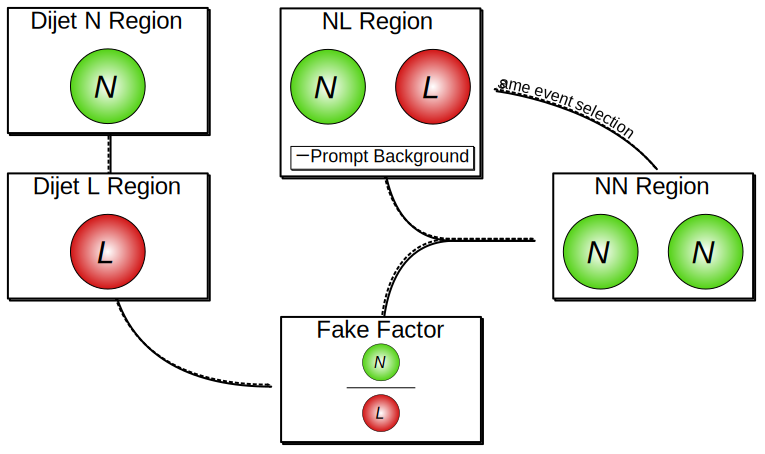
\includegraphics[width=.8\textwidth]{figs/ssww_13tev/backgrounds/ff/fake_factor}
  \caption{Graphical representation of how the fake factor method is used to estimate the fake background in a given $NN$ region.}
  \label{fig:ssww13tev_ff_apply}
\end{figure}

%---------------------------------------------------------------------------------------------
%
%---------------------------------------------------------------------------------------------
\subsubsection{The fake-factor with $\ptcone$}\label{ssww13tev:ff_method_ptcone}
When a jet produces a non-prompt lepton, that lepton only carries a fraction of the underlying jet's total momentum.
Due to the isolation cut applied to the nominal leptons, they typically carry a much larger percentage of the underlying jet momentum than the loose leptons. %(which are allowed to fail this criteria). 
Since the isolation essentially sets a limit on the amount of detector activity allowed around the lepton, if other nearby particles carried a significant amount of momentum, the lepton would likely fail this cut.

This discrepancy in the underlying jet momentum fraction can cause problems in the calculation of the fake-factor $f$.
Consider the case where two separate events have jets of identical momentum, but one produces a non-prompt lepton that passes the nominal selection, and the other produces a non-prompt lepton that passes the loose selection.
The loose lepton on average will have lower $\pt$ than the nominal lepton despite both originating from jets with the same momentum.
This can be seen explicitly when comparing the $\pt$ of a muon to its associated truth jet:
\begin{equation}
\Delta\pt(\mu,j) = \frac{\pt(j)-\pt(\mu)}{\pt(j)+\pt(\mu)}
\label{eq:ssww13tev_ff_deltapt}
\end{equation}
Since muons are not included in the jet reconstruction algorithm, $\Delta\pt$ approximates the momentum of the muon compared to the rest of the jet.
For muons that carry more than 50\% of the jet's momentum, $\Delta\pt$ will be negative and vice-versa.
The $\Delta\pt$ distributions for nominal and loose muons in $t\bar{t}$ MC events is shown Figure~\ref{fig:ssww13tev_ff_deltapt}, where a $50\gev$ jet on average corresponds to a $35\gev$ nominal muon and a $20\gev$ loose muon\footnote{To better illustrate the point, here the muon is added back into the jet $\pt$, and the corresponding muon $\pt$ is obtained via $\Delta\pt(\mu,j) = \frac{\big(\pt(j)-\pt{\mu}\big)-\pt(\mu)}{\big(\pt(j)-\pt(\mu)\big)+\pt(\mu)} = \frac{\pt(j)-2\pt(\mu)}{\pt(j)}$.}.

\begin{figure}[htbp]
  \centering
  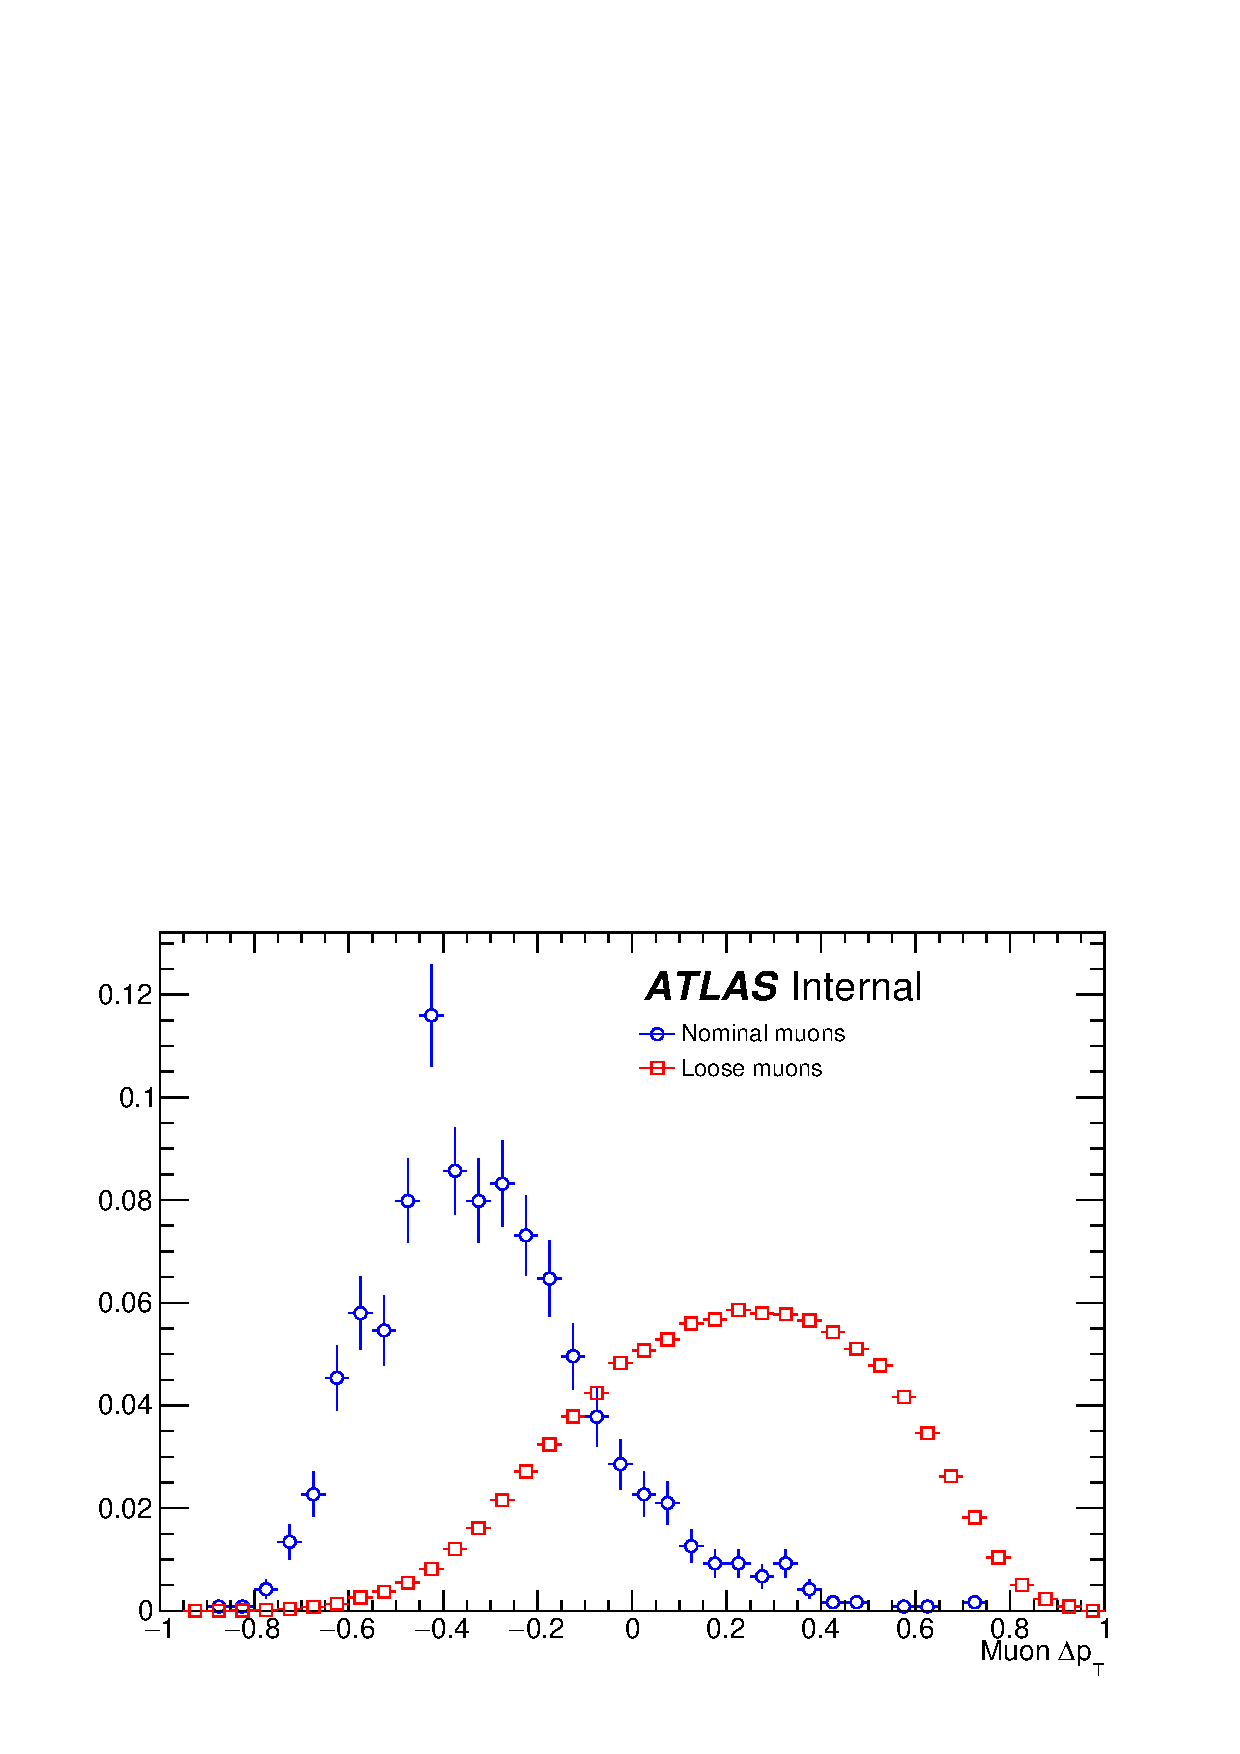
\includegraphics[width=.6\textwidth]{figs/ssww_13tev/backgrounds/ff/deltapt_ttbar}
  \caption{$\Delta\pt$ distributions for nominal (blue) and loose (red) muons in simulated $t\bar{t}$ events.  Each muon has been matched to a truth-level jet.  Both distributions are normalized to unit area.}
  \label{fig:ssww13tev_ff_deltapt}
\end{figure}

Since the default fake-factor defined in Equation~\ref{eq:ssww13tev_ff_default_binned} is binned in lepton $\pt$, within a given bin, the underlying jet $\pt$ spectrum can differ substantially between the numerator and the denominator.
Additionally, these differences can vary depending on the process producing the non-prompt leptons or on the specific kinematic selections of the signal or control regions where the fake-factor is applied.

Fortunately, the majority of the jet momentum not carried by the non-prompt lepton (excluding neutrinos) can be recovered using isolation variables.
A track-based isolation is chosen, referred to as $\ptcone$, and it contains the sum of the $\pt$ of all particle tracks originating from the primary vertex within a cone of $\deltar < 0.3$ around the lepton.
Thus, the sample of loose leptons in the denominator of the fake-factor calculation is binned in $\ptptcone$ rather than simply lepton $\pt$.
Adding the isolation cone greatly reduces the difference in the fraction of the underlying jet momentum carried by the nominal and loose leptons.
To check this, a new $\Delta\pt$ is calculated between a lepton and its matched truth jet, where the truth jet $\pt$ has been corrected to include all muons within a cone of $\deltar < 0.4$:
\begin{equation}
\pt(j) = \pt(j_{\textrm{truth}})+\sum\limits_{\deltar < 0.4}\pt(\mu_{\textrm{truth}})
\label{eq:ssww13tev_ff_jet_corr}
\end{equation}
The $\Delta\pt$ distributions comparing $\pt$ and $\ptptcone$ for nominal and loose leptons using the corrected jet $\pt$ are found in Figure~\ref{fig:ssww13tev_ff_deltapt_ptcone}, and better agreement is seen between the numerator (nominal) and denominator (loose with $\ptptcone$) distributions.

\begin{figure}[htbp]
  \centering
  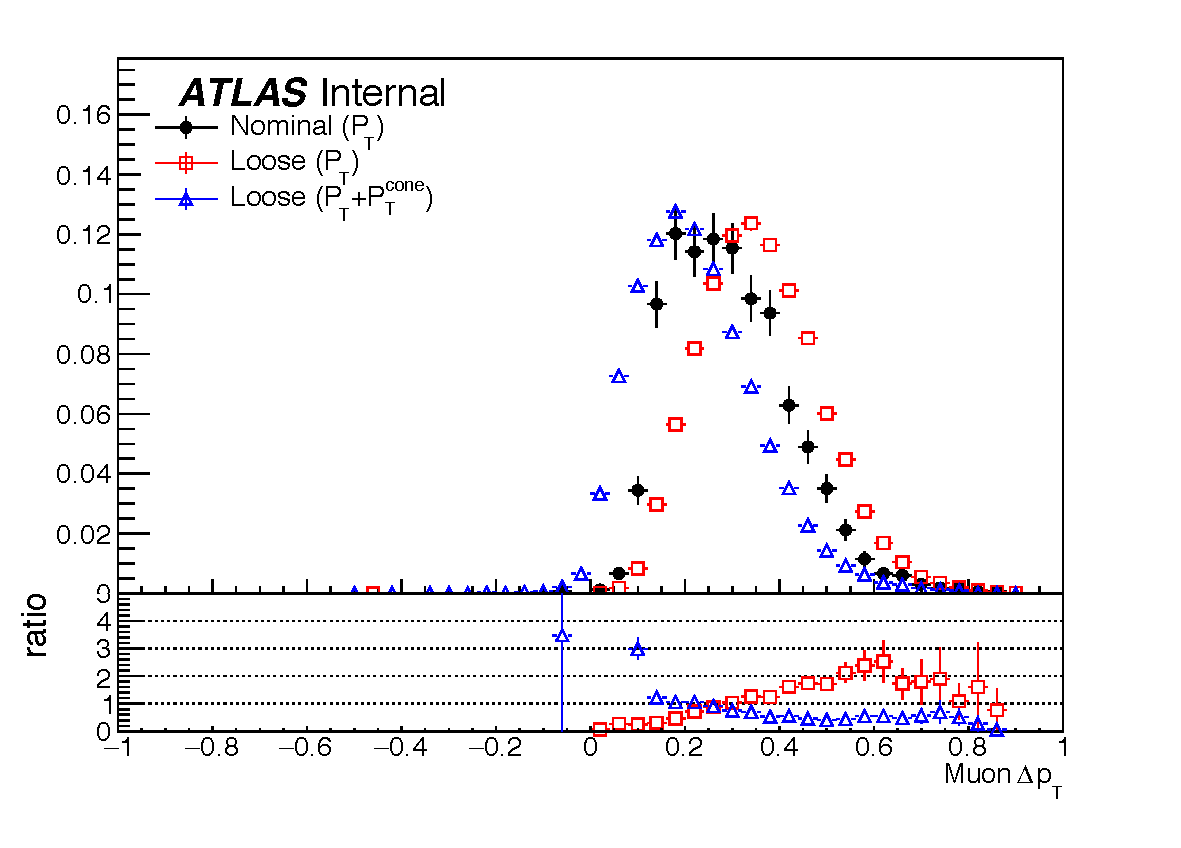
\includegraphics[width=.6\textwidth]{figs/ssww_13tev/backgrounds/ff/dpt_muon_ttbar}\\
  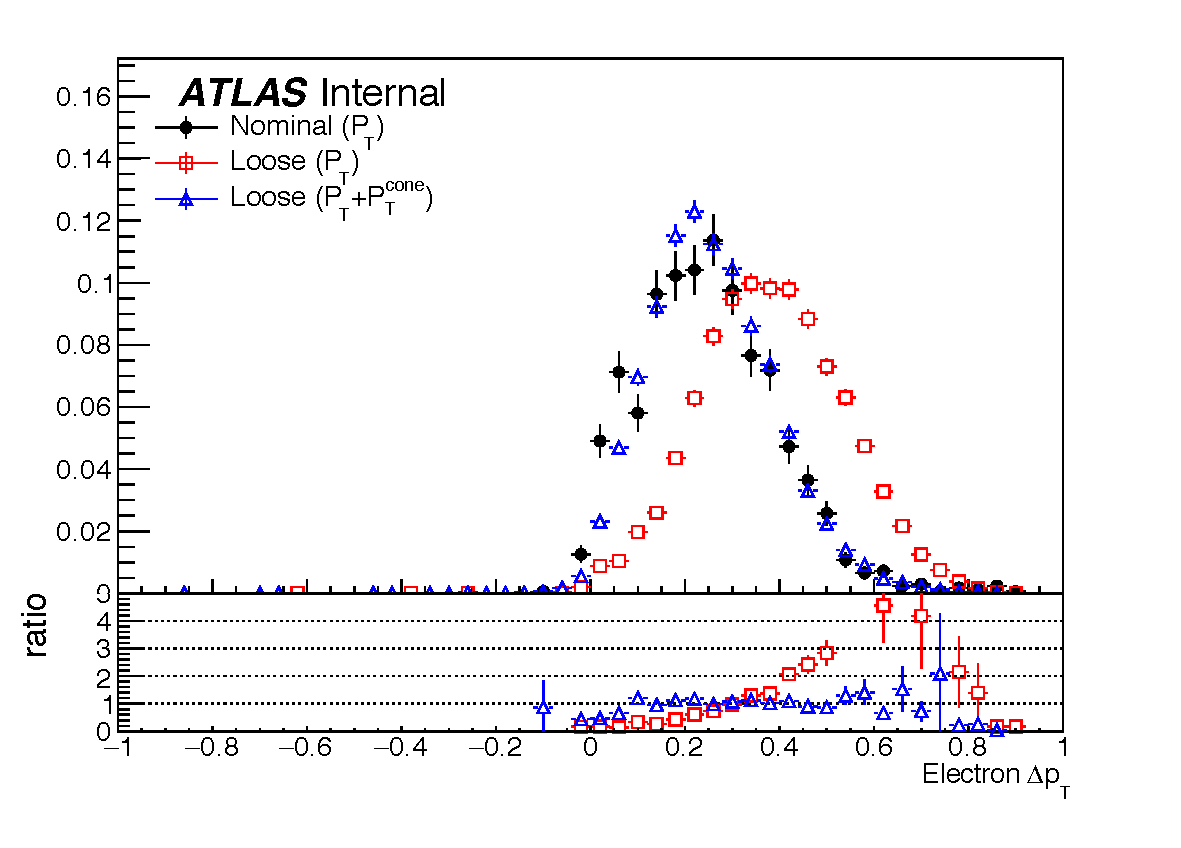
\includegraphics[width=.6\textwidth]{figs/ssww_13tev/backgrounds/ff/dpt_elec_ttbar}
  \caption{$\Delta\pt$ distributions for muons (top) and electrons (bottom) in simulated $t\bar{t}$ events.  Each lepton has been matched to a truth-level jet, and that truth jet has had its $\pt$ corrected to include all truth muons within a cone of $\deltar < 0.4$.  The nominal leptons are in black. $\Delta\pt$ is calculated for the loose leptons using $\pt$ (red) and $\ptptcone$ (blue).}
  \label{fig:ssww13tev_ff_deltapt_ptcone}
\end{figure}

The numerator remains binned in lepton $\pt$, due to the fact that it is meant to mirror the signal region as closely as possible, and the signal lepton selection does not use $\ptptcone$.
The impact of this is expected to be negligible due to the $\ptcone$ isolation being small for signal leptons, as shown for muons in Figure~\ref{fig:ssww13tev_ff_ptcone_muons}.
Finally, the fake-factor $f$ becomes:

\begin{equation}
%f_b = \frac{N_{\textrm{nominal}}^b(\pt)}{N_{\textrm{loose}}^b(\ptptcone)}
f(b) = \frac{N_{\textrm{nominal}}\big(b(\pt)\big)}{N_{\textrm{loose}}\big(b(\ptptcone)\big)}
\label{eq:ssww13tev_ff_ptcone_binned}
\end{equation}

\begin{figure}[htbp]
  \centering
  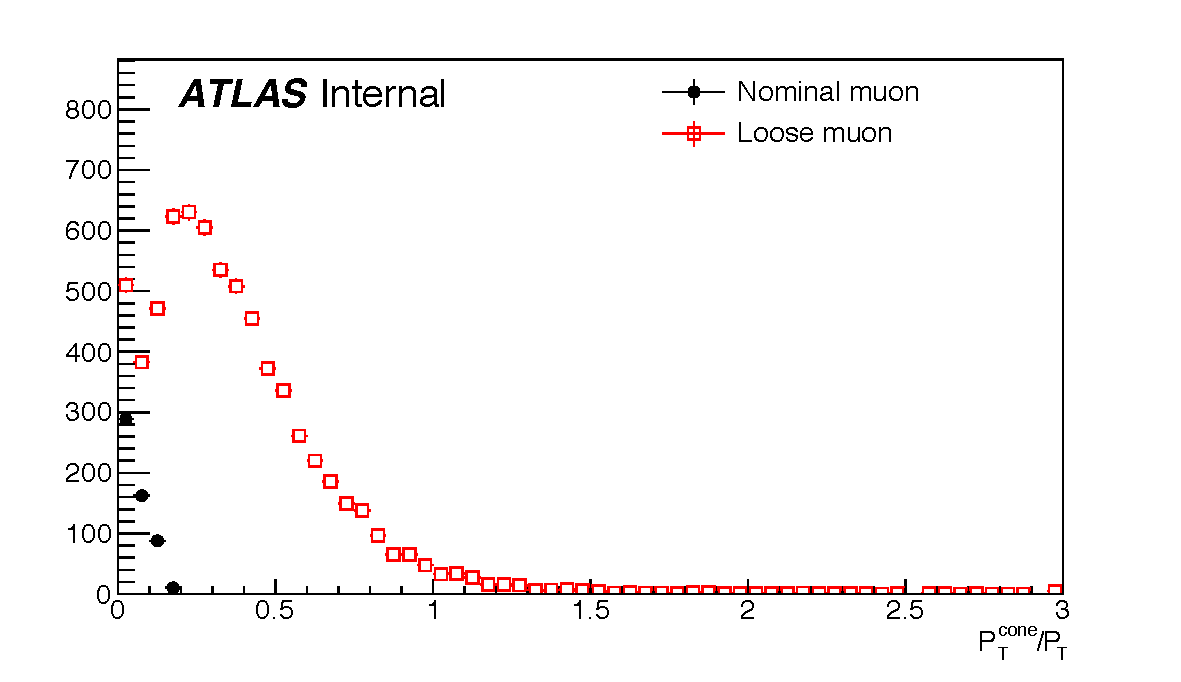
\includegraphics[width=.6\textwidth]{figs/ssww_13tev/backgrounds/ff/ptcone_muon_ttbar}
  \caption{Distributions of $\ptcone/\pt$ for nominal (black) and loose (red) muons in simulated $t\bar{t}$ events.}
  \label{fig:ssww13tev_ff_ptcone_muons}
\end{figure}

%---------------------------------------------------------------------------------------------
%
%---------------------------------------------------------------------------------------------
\subsubsection{Application of the fake-factor}\label{ssww13tev:ff_implementation}
The fake-factor itself is measured from a sample data events passing a dijet selection requiring exactly one lepton (either passing the nominal or loose selections) and at least one jet.
The leading jet must also be $b$-tagged and approximately back-to-back with the lepton in order to enhance non-prompt lepton contributions while reducing contributions from processes involving $W$ and $Z$ bosons.
$W$ boson events are further suppressed by requiring the sum of the $\met$ and the transverse mass of the lepton to be less than $50\gev$.
The full event selection for the dijet region is summarized in Table~\ref{tab:ssww13tev_dijet_cr}.

\begin{table}[hbtp]
  \centering
  \begin{tabular}{c}
    Dijet event selection \\
    \hline\hline
    Event preselection\\
    Exactly one lepton with $\pt > 15\gev$\\
    $N_{\textrm{jet}} > 0$ \\
    Leading jet is $b$-tagged \\
    $\pt^{\textrm{lead.\ jet}} > 25\gev$\\
    $\pt^{\textrm{lead.\ jet}} > 30\gev$ if $|\eta_j| > 2.5$ \\
    $|\Delta\phi(l,\textrm{lead.\ jet})| > 2.8$ \\
    $m_{\textrm{T}}(l,\met) + \met < 50\gev$ \\
    \hline
  \end{tabular}
  \caption{Event selection for the dijet region used for calculating the fake-factor. The selected lepton can pass either the nominal (signal) or loose selections.  In the case of the nominal leptons, the $\pt > 27\gev$ requirement is replaced with $\pt > 15\gev$.}
  \label{tab:ssww13tev_dijet_cr}
\end{table}

The numerator sample is constructed from dijet events in which the lepton passes the nominal (signal) selection and is binned in the lepton $\pt$.
Similarly, the denominator sample is made up of the remaining dijet events where the lepton passes the loose selection and is binned in the lepton $\ptptcone$.
The nominal and loose leptons pass the signal selection\footnote{The $\pt > 27\gev$ cut in the signal lepton selection is dropped in favor of the $\pt > 15\gev$ requirement in the dijet selection.} and loose selection, respectively, defined earlier in Table~\ref{tab:ssww13tev_muon_selection} for muons and Table~\ref{tab:ssww13tev_elec_selection} for electrons.
Backgrounds from $W$+jets, $Z$+jets, $t\bar{t}$, and single top processes are estimated from MC simulations requiring one lepton to be prompt using the truth information; these contributions are subtracted from the dijet data.
The fake-factor is then calculated using Equation~\ref{eq:ssww13tev_ff_ptcone_binned} for muons and for central and forward electrons separately.
The muon fake-factor is shown in Figure~\ref{fig:ssww13tev_ff_muon}, and the two electron fake-factors are shown in Figure~\ref{fig:ssww13tev_ff_elec}.
The numerical values of the fake-factors, including their systematic uncertainties which will be discussed in Section~\ref{ssww13tev:ff_systematics}, are listed in Table~\ref{tab:ssww13tev_ff}.

\begin{figure}[htbp]
  \centering
  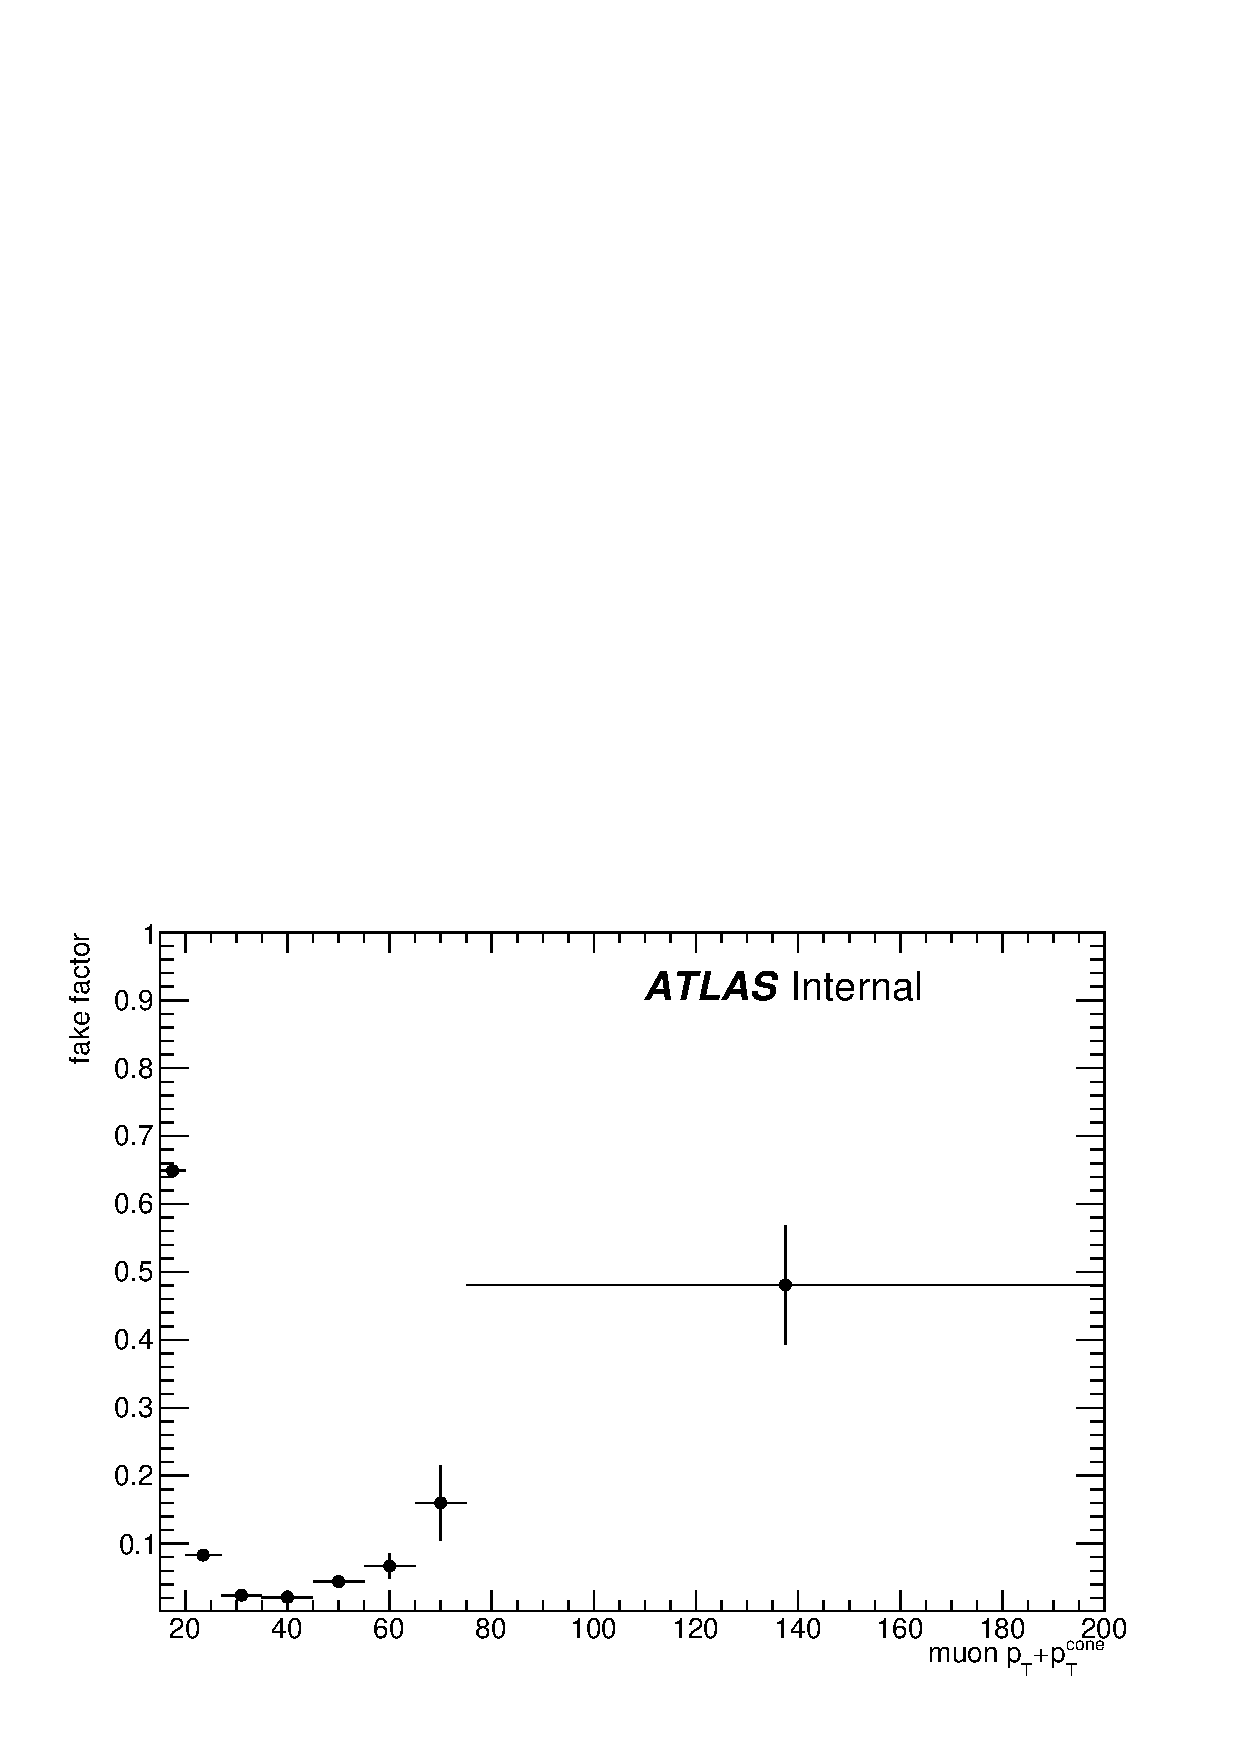
\includegraphics[width=.6\textwidth]{figs/ssww_13tev/backgrounds/ff/muon_ff}
  \caption{The measured fake-factor as a function of muon $\ptptcone$.  The error bars represent the statistical uncertainty only.}
  \label{fig:ssww13tev_ff_muon}
\end{figure}

\begin{figure}[htbp]
  \centering
  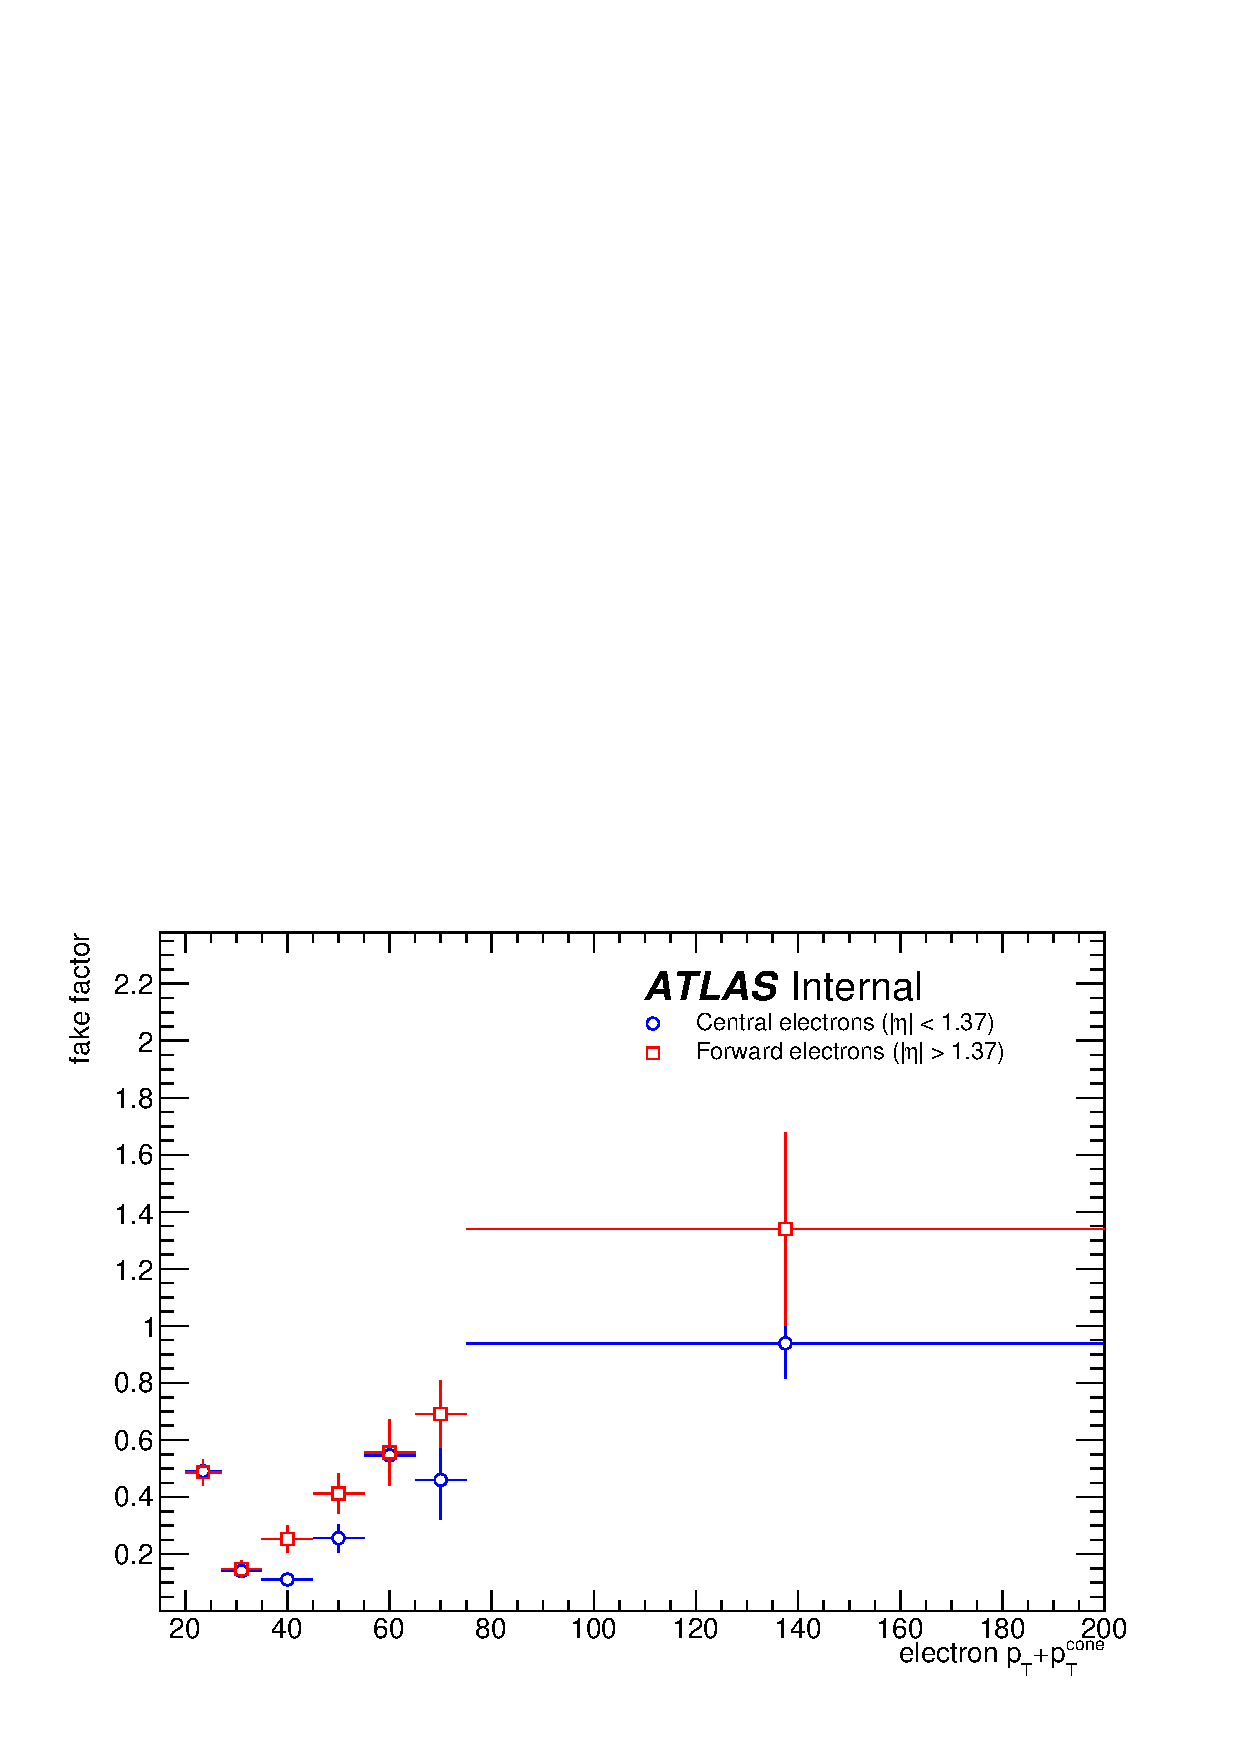
\includegraphics[width=.6\textwidth]{figs/ssww_13tev/backgrounds/ff/elec_ff}
  \caption{The measured fake-factor as a function of electron $\ptptcone$ in the central ($|\eta|<1.37$, blue) and forward ($|\eta| > 1.37$, red) regions of the detector.  The error bars represent the statistical uncertainty only.}
  \label{fig:ssww13tev_ff_elec}
\end{figure}

In order to properly account for the denominator being binned in $\ptptcone$, special care needs to be taken when estimating the fake background from the $NL$ regions.
For the purposes of the fake-factor calculation, it is perhaps more intuitive to consider a loose \emph{object} with $\pt=\ptptcone$ instead of simply a loose \emph{lepton}, as the lepton and the underlying jet are treated as a whole with this method.
When the lepton $\pt$ cuts required by a particular signal or control region are applied to nominal and loose leptons, the cut is applied to the $\pt$ of the nominal lepton and to the $\ptptcone$ of the loose object.
Similarly, when looking up the fake-factor weight for a given $NL$ event, the value taken from the bin corresponding to the $\ptptcone$ of the loose object.
Finally, when applying the weight to the event, $\ptptcone$ is assigned as the $\pt$ of the loose object.
This can be visualized by referring back to Figure~\ref{fig:ssww13tev_ff_apply}; every time a loose lepton is used (the red circles in the Figure), $\ptptcone$ is used in place of $\pt$.
%Figure~\ref{fig:ssww13tev_ff_application} contains a graphical representation of this procedure.

%\begin{figure}[htbp]
%  \centering
%  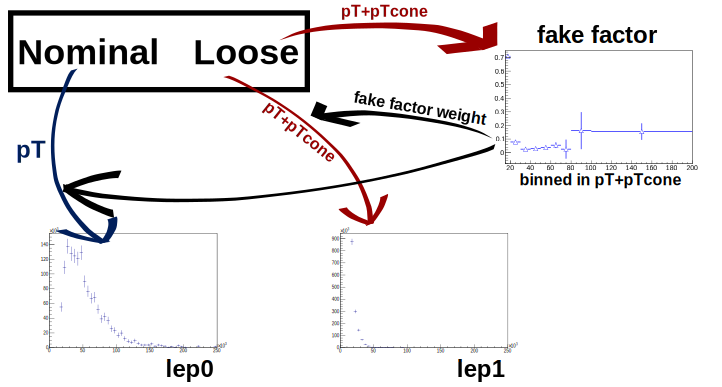
\includegraphics[width=.95\textwidth]{figs/ssww_13tev/backgrounds/ff/apply_ff}
%  \caption{Graphical representation of the fake-factor application using $\ptptcone$.  The value of $\ptptcone$ for the loose lepton is used to ``look up'' the fake-factor weight which is then applied to the event.  The loose lepton's $\pt$ becomes $\ptptcone$ for the purpose of the fake background estimation. \TODO{Update figure to match style of Fig.~\ref{fig:ssww13tev_ff_apply}.}}
%  \label{fig:ssww13tev_ff_application}
%\end{figure}

Finally, it should be noted that the addition of $\ptcone$ to the loose object may cause the loose leptons in the denominator sample to migrate into higher bins.
This results in an overall decrease in the number of loose objects in the lower $\ptptcone$ bins due to there not being additional leptons at lower $\pt$ to replace them.
Since the fake-factor is a ratio of the number of events in a bin, this effect causes the first few bins of the fake-factor to increase, as can be seen clearly in Figure~\ref{fig:ssww13tev_ff_muon}.
However, the signal and control regions (and their corresponding $NL$ regions) contain a $\pt > 27\gev$ cut that prevents these migrations from negatively impacting the fake estimation.

%---------------------------------------------------------------------------------------------
%
%---------------------------------------------------------------------------------------------
\subsubsection{Systematic uncertainties}\label{ssww13tev:ff_systematics}
Four sources of systematic uncertainty are considered: the dijet event selection, the prompt background subtraction, the jet flavor composition, and residual dependence on the underlying jet $\pt$ spectrum.
In order to measure the impact of these systematics, new fake-factors are computed with each of the systematic variations and the differences from the nominal values are taken as the uncertainty.
\begin{enumerate}
\item In order to estimate uncertainties due to the dijet selection, the cut on $M_{\textrm{T}}+\met$ is varied by $\pm5\gev$, the jet-lepton separation $\Delta\phi(l,j)$ by $\pm 0.1$, and the jet $\pt$ cut by $+5\gev$.
\item To estimate the systematic uncertainty on the prompt background subtraction, the MC prediction in a $W$+jets control region is compared to data.  The discrepancy between data and MC is found to be approximately 10\%~\cite{2018.ssww-13tev-atlas-support}.  Therefore, the prompt background used for the subtraction is scaled up and down by $\pm 10\%$.
\item The difference in the jet flavor composition between the dijet events and the events in the $NL$ regions can affect the accuracy of the fake background estimation.  The dijet sample is dominated by light jets, while the $NL$ regions tend to be dominated by heavy flavor from $t\bar{t}$.  To account for this, the fake-factor is computed with a $b$-jet veto.
\item To measure any residual dependence on the underlying jet $\pt$ spectrum, the leading jet $\pt$ distribution is reweighted to match the $\pt$ spectrum of truth jets that produce fake leptons in MC simulations.  This results in an increase in the number of nominal and loose leptons at high momentum~\cite{2018.ssww-13tev-atlas-support}.
\end{enumerate}
%An overall uncertainty of 50\% is assigned to the fake background estimation in $\mu^{\pm}\mu^{\pm}$ events, and between 40\% to 90\% for $e^{\pm}e^{\pm}$ and $\mu^{\pm}e^{\pm}$ events, including both statistical and systematic effects.

\begin{figure}[htbp]
  \centering
  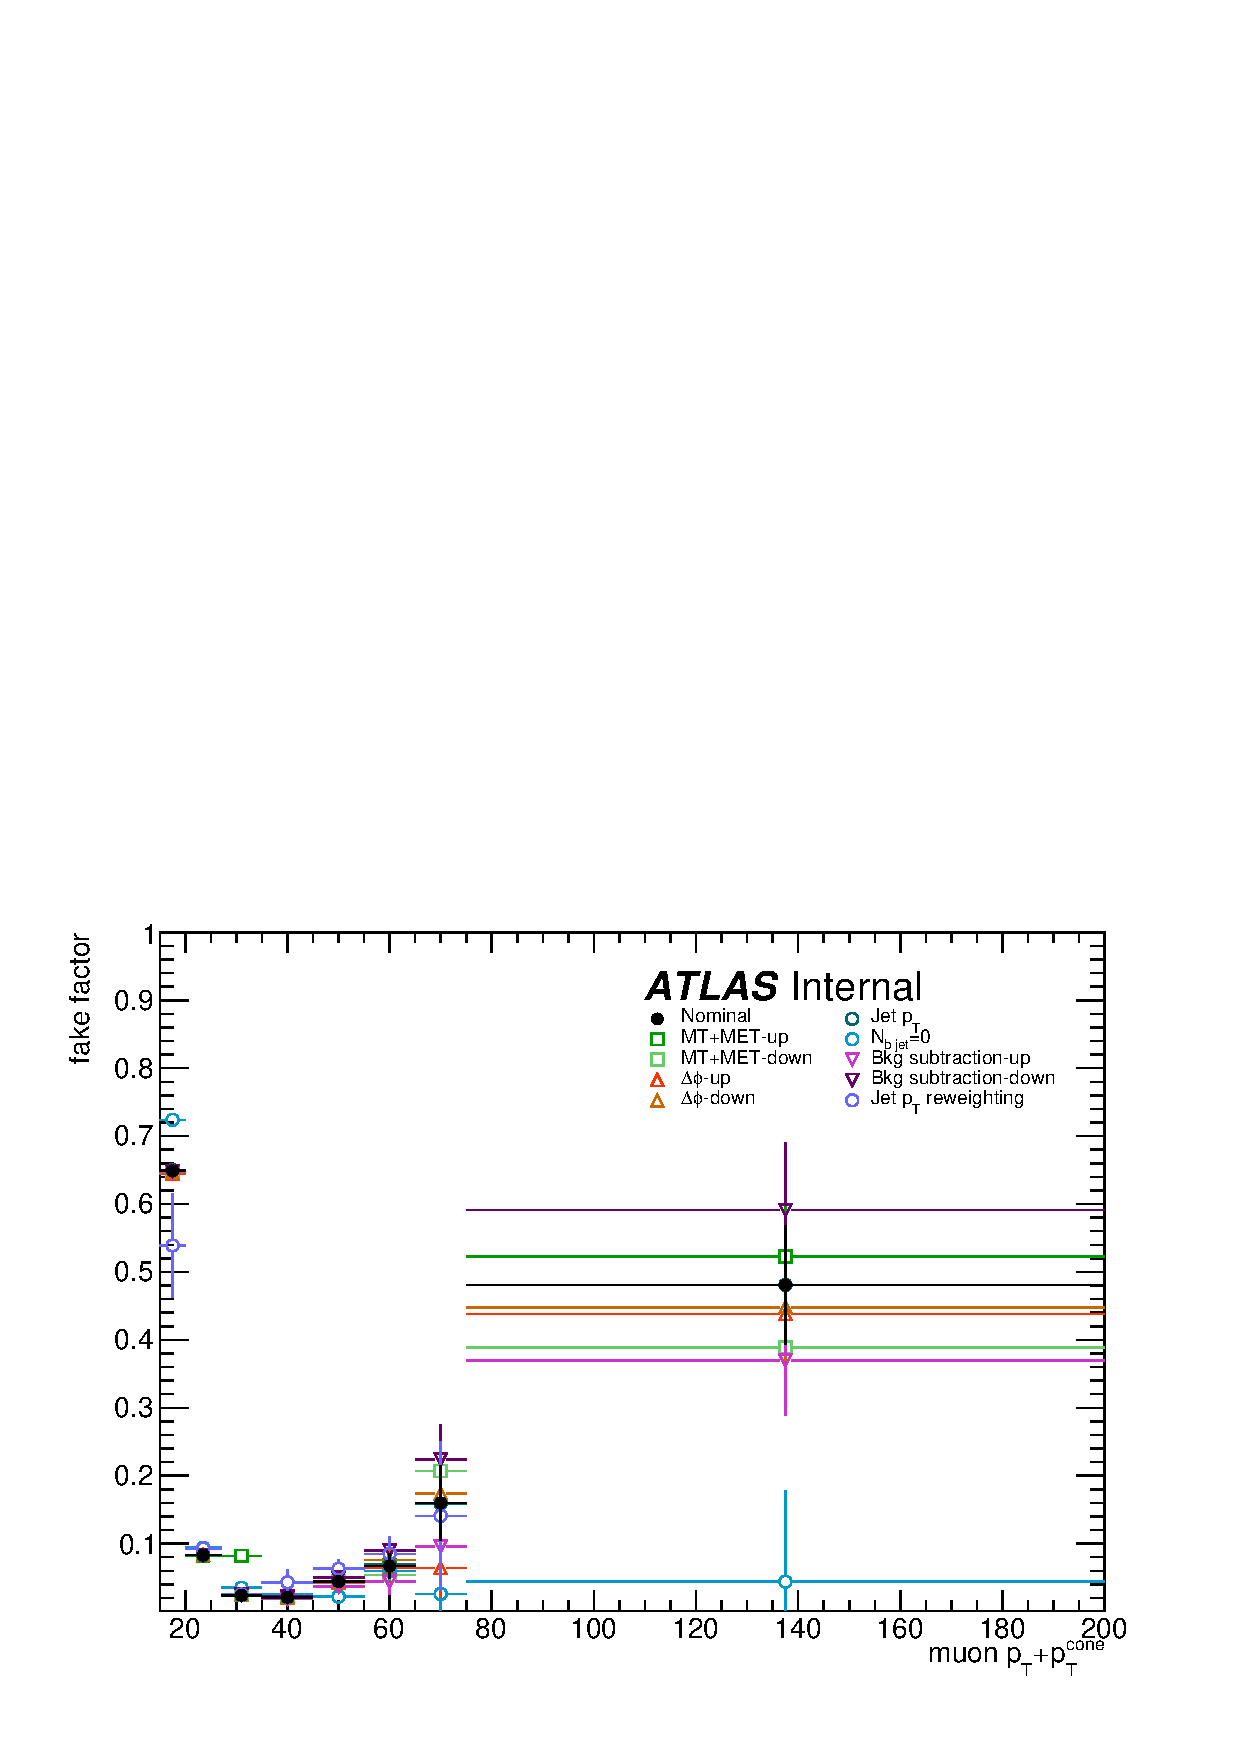
\includegraphics[width=.6\textwidth]{figs/ssww_13tev/backgrounds/ff/muon_ff_sys}
  \caption{Systematic variations in the fake-factor as a function of muon $\ptptcone$.  The individual fake-factors obtained for each systematic variation are displayed with their statistical uncertainties.}
  \label{fig:ssww13tev_ff_muon_sys}
\end{figure}

\begin{figure}[htbp]
  \centering
  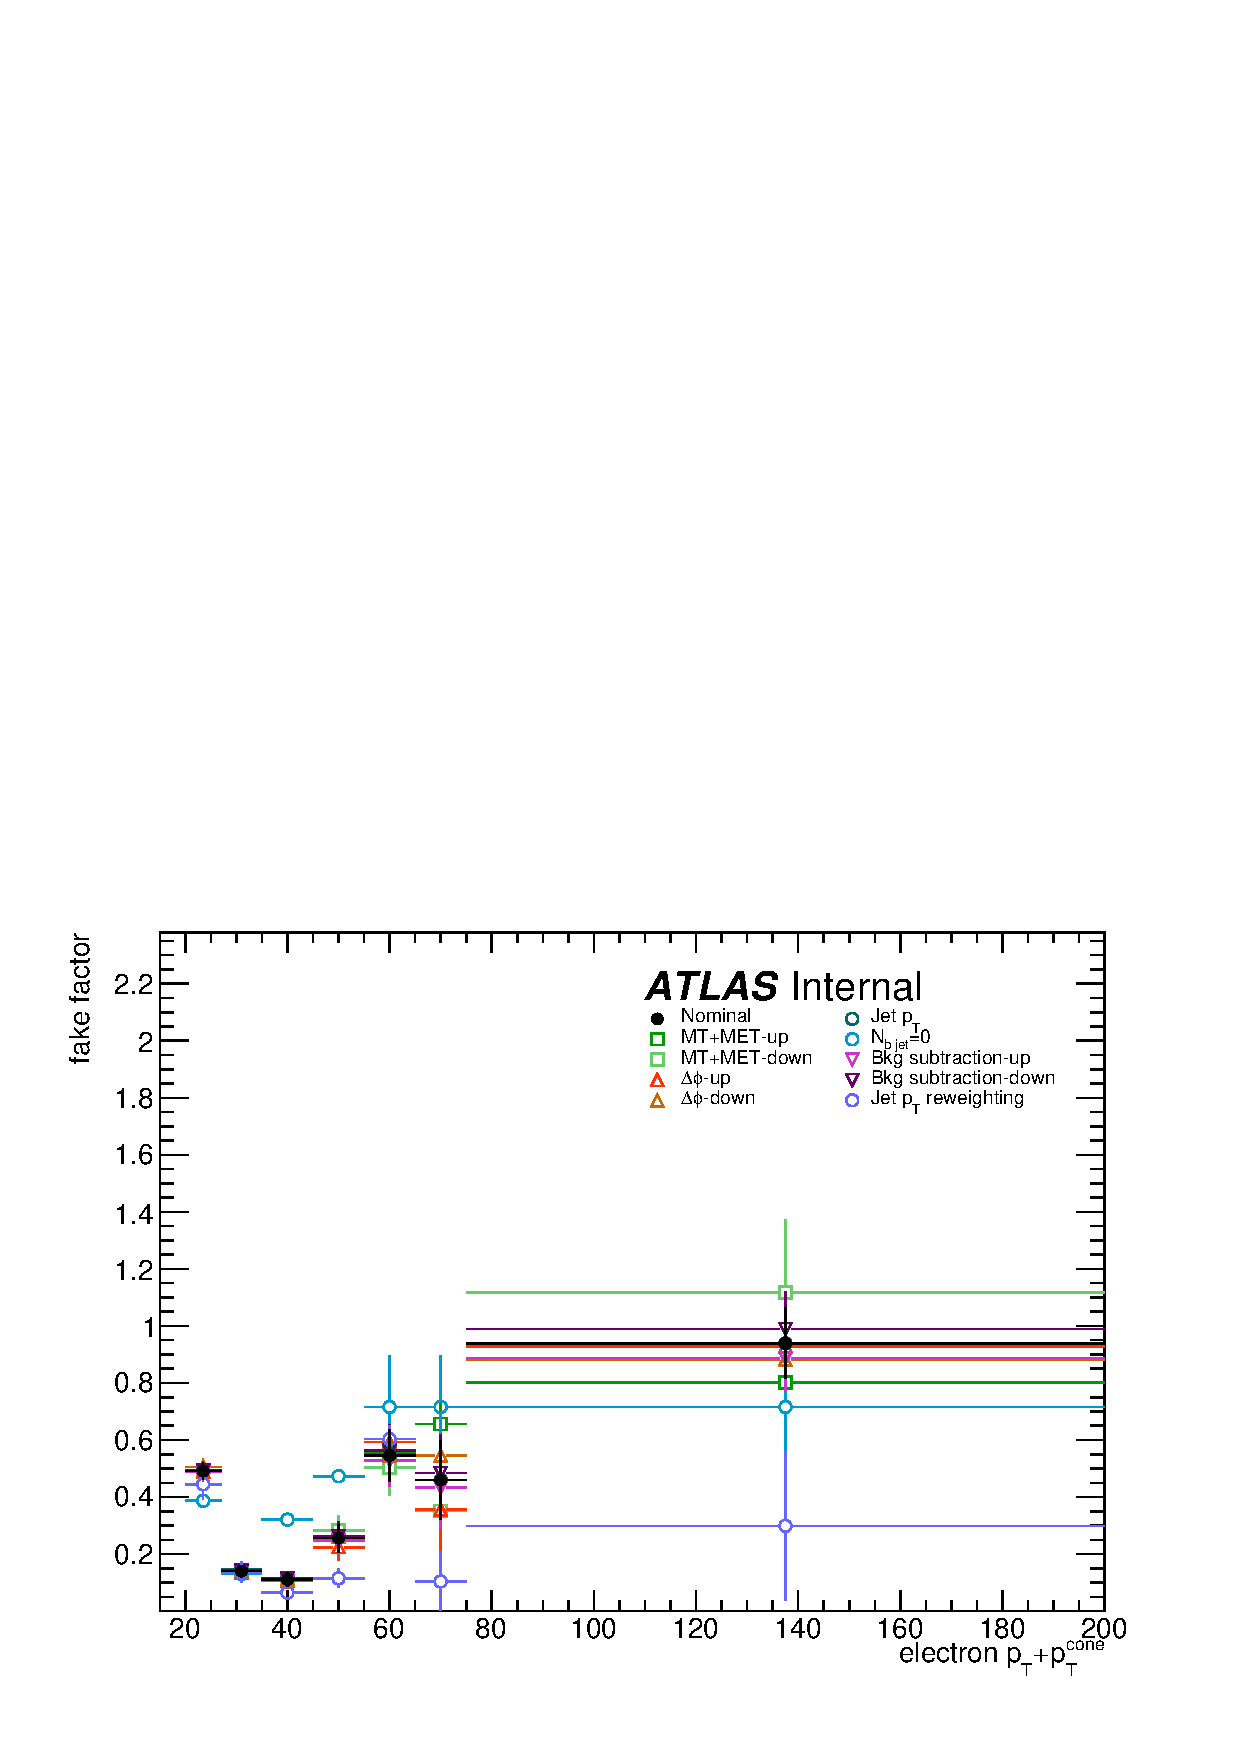
\includegraphics[width=.6\textwidth]{figs/ssww_13tev/backgrounds/ff/elec_central_ff_sys}\\
  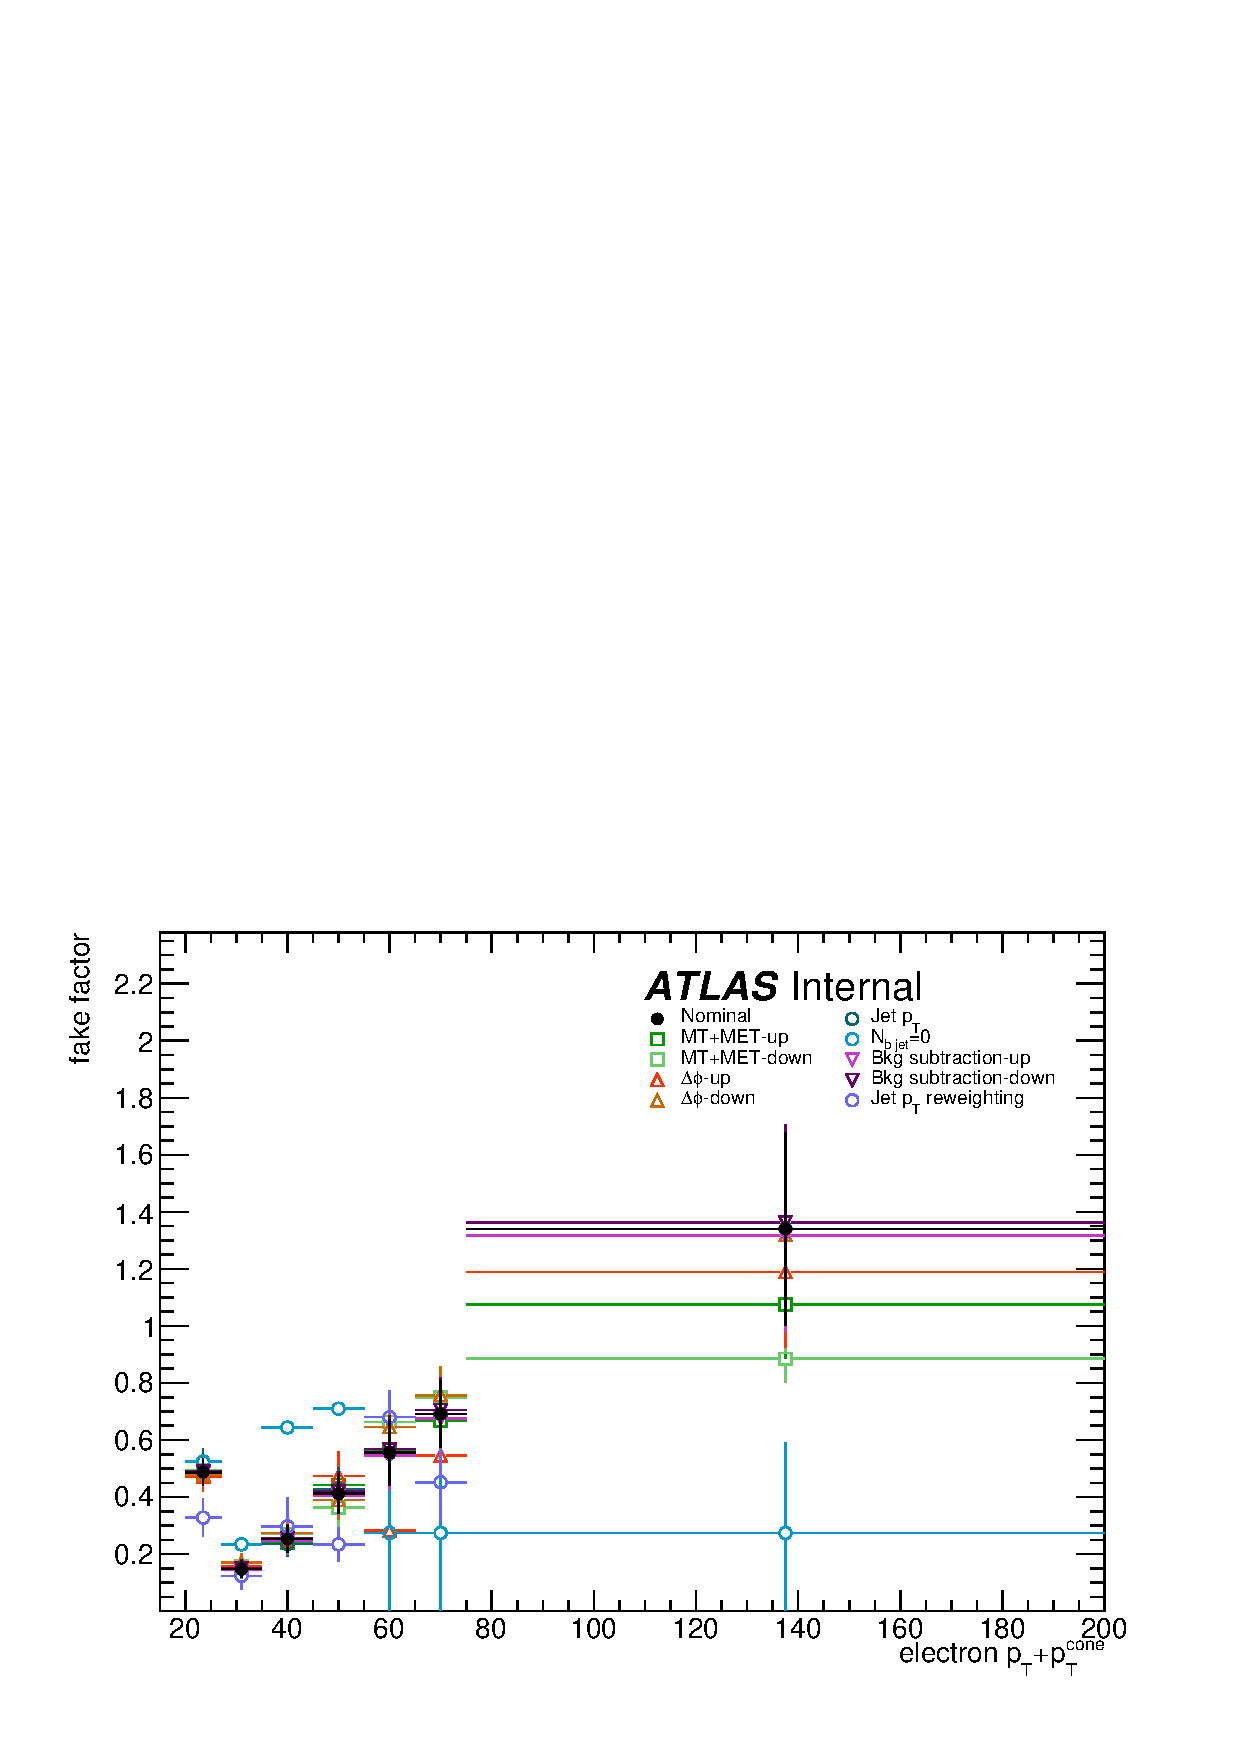
\includegraphics[width=.6\textwidth]{figs/ssww_13tev/backgrounds/ff/elec_forward_ff_sys}
  \caption{Systematic variations in the fake-factor as a function of electron $\ptptcone$ in the central ($|\eta|<1.37$, top) and forward ($|\eta| > 1.37$, bottom) regions of the detector.  The individual fake-factors obtained for each systematic variation are displayed with their statistical uncertainties.}
  \label{fig:ssww13tev_ff_elec_sys}
\end{figure}

\begin{table}[hbtp]
  \begin{subtable}{\linewidth}
  \centering
  \resizebox{1.0\textwidth}{!}{
  \begin{tabular}{l|cccccccc}
    fake-factor & $\pt$  [15, 20]      &  $\pt$[20, 27]       &    $\pt$[27, 35]     &    $\pt$[35, 45]     &    $\pt$[45, 55]     &    $\pt$[55, 65]     &    $\pt$[65, 75]     &    $\pt$[75, 200]    \\ \hline\hline
    nominal     & 0.649 $\pm$ 0.007  & 0.083 $\pm$ 0.002 & 0.024 $\pm$ 0.002  & 0.021 $\pm$ 0.003   & 0.044 $\pm$ 0.007   & 0.067 $\pm$ 0.018  & 0.160 $\pm$ 0.055   & 0.481 $\pm$ 0.088 \\ \hline
    \multirow{2}{*}{MT+MET}   & 0.649 $\pm$ 0.007  & 0.082 $\pm$ 0.002   & 0.082 $\pm$ 0.002    & 0.020 $\pm$ 0.003    & 0.045 $\pm$ 0.007 & 0.068 $\pm$ 0.018 & 0.207 $\pm$ 0.062 & 0.523 $\pm$ 0.086 \\
    & 0.648 $\pm$ 0.007 & 0.083 $\pm$ 0.003 & 0.024 $\pm$ 0.002 & 0.022 $\pm$ 0.004 & 0.044 $\pm$ 0.007 & 0.054 $\pm$ 0.020 & 0.207 $\pm$ 0.060 & 0.389 $\pm$ 0.081 \\ \hline
    \multirow{2}{*}{$\Delta\phi(\ell,j)$}    & 0.645 $\pm$ 0.008 & 0.083 $\pm$ 0.003 & 0.024 $\pm$ 0.002 & 0.021 $\pm$ 0.004 & 0.045 $\pm$ 0.008 & 0.064 $\pm$ 0.021 & 0.064 $\pm$ 0.058 & 0.438 $\pm$ 0.092 \\
      & 0.646 $\pm$ 0.006 & 0.083 $\pm$ 0.002 & 0.024 $\pm$ 0.002 & 0.020 $\pm$ 0.003 & 0.043 $\pm$ 0.006 & 0.076 $\pm$ 0.017 & 0.174 $\pm$ 0.050 & 0.448 $\pm$ 0.078 \\ \hline
    Jet $\pt$        & 0.650 $\pm$ 0.007 & 0.083 $\pm$ 0.002 & 0.024 $\pm$ 0.002 & 0.021 $\pm$ 0.003 & 0.045 $\pm$ 0.007 & 0.069 $\pm$ 0.018 & 0.159 $\pm$ 0.018 & 0.481 $\pm$ 0.088 \\ \hline 
    $N_{\textrm{b-jet}} = 0$      & 0.724 $\pm$ 0.003 & 0.094 $\pm$ 0.001 & 0.035 $\pm$ 0.001 & 0.025 $\pm$ 0.002 & 0.022 $\pm$ 0.004 & 0.060 $\pm$ 0.015 & 0.026 $\pm$ 0.053 & 0.044 $\pm$ 0.134 \\ \hline 
    \multirow{2}{*}{Bkg. subtraction}   & 0.648 $\pm$ 0.007 & 0.083 $\pm$ 0.002 & 0.024 $\pm$ 0.002 & 0.019 $\pm$ 0.003 & 0.037 $\pm$ 0.007 & 0.044 $\pm$ 0.019 & 0.096 $\pm$ 0.062 & 0.370 $\pm$ 0.082 \\
    & 0.649 $\pm$ 0.007 & 0.083 $\pm$ 0.002 & 0.025 $\pm$ 0.002 & 0.022 $\pm$ 0.003 & 0.050 $\pm$ 0.007 & 0.090 $\pm$ 0.017 & 0.224 $\pm$ 0.052 & 0.591 $\pm$ 0.099 \\ \hline 
   Jet $\pt$ Reweight & 0.539 $\pm$ 0.077 & 0.093 $\pm$ 0.007 & 0.025 $\pm$ 0.004 & 0.043 $\pm$ 0.019 & 0.063 $\pm$ 0.014 & 0.085 $\pm$ 0.025 & 0.141 $\pm$ 0.110 & 1.962 $\pm$ 0.492 \\ 
    \hline
  \end{tabular}
  }
  \caption{fake-factor for muons.}
  \end{subtable}

  \vspace{10mm}

  \begin{subtable}{\linewidth}
  \centering
  \resizebox{1.0\textwidth}{!}{
  \begin{tabular}{l|cccccccc}
    fake-factor   &  $\pt$[20, 27]       &    $\pt$[27, 35]     &    $\pt$[35, 45]     &    $\pt$[45, 55]     &    $\pt$[55, 65]     &    $\pt$[65, 75]     &    $\pt$[75, 200]    \\ \hline\hline
    nominal     & 0.491 $\pm$ 0.031 & 0.140 $\pm$ 0.020 & 0.111 $\pm$ 0.023 & 0.256 $\pm$ 0.049 & 0.546 $\pm$ 0.091 & 0.460 $\pm$ 0.140 & 0.939 $\pm$ 0.125 \\ \hline
    \multirow{2}{*}{MT+MET}   & 0.493 $\pm$ 0.030 & 0.138 $\pm$ 0.019 & 0.115 $\pm$ 0.022 & 0.261 $\pm$ 0.045 & 0.559 $\pm$ 0.084 & 0.656 $\pm$ 0.091 & 0.802 $\pm$ 0.016 \\
                              & 0.488 $\pm$ 0.032 & 0.137 $\pm$ 0.020 & 0.110 $\pm$ 0.025 & 0.283 $\pm$ 0.053 & 0.503 $\pm$ 0.097 & 0.351 $\pm$ 0.149 & 1.117 $\pm$ 0.255 \\ \hline
    \multirow{2}{*}{$\Delta\phi(\ell,j)$}  & 0.489 $\pm$ 0.035 & 0.134 $\pm$ 0.021 & 0.105 $\pm$ 0.025 & 0.224 $\pm$ 0.048 & 0.593 $\pm$ 0.093 & 0.356 $\pm$ 0.144 & 0.928 $\pm$ 0.177 \\ 
     & 0.506 $\pm$ 0.029 & 0.140 $\pm$ 0.018 & 0.111 $\pm$ 0.022 & 0.260 $\pm$ 0.046 & 0.545 $\pm$ 0.084 & 0.546 $\pm$ 0.120 & 0.882 $\pm$ 0.103  \\  \hline
    Jet $\pt$    & 0.493 $\pm$ 0.032 & 0.146 $\pm$ 0.021 & 0.115 $\pm$ 0.024 & 0.259 $\pm$ 0.049 & 0.550 $\pm$ 0.091 & 0.460 $\pm$ 0.140 & 0.939 $\pm$ 0.125 \\ \hline 
    $N_{\textrm{b-jet}} = 0$      & 0.387 $\pm$ 0.009 & 0.130 $\pm$ 0.008 & 0.321 $\pm$ 0.012 & 0.473 $\pm$ 0.015 & 0.716 $\pm$ 0.180 & 0.716 $\pm$ 0.180 & 0.716 $\pm$ 0.180 \\ \hline 
    \multirow{2}{*}{Bkg. subtraction}   & 0.488 $\pm$ 0.031 & 0.138 $\pm$ 0.020 & 0.106 $\pm$ 0.023& 0.248 $\pm$ 0.049 & 0.529 $\pm$ 0.092 & 0.434 $\pm$ 0.143 & 0.888 $\pm$ 0.115 \\ 
      & 0.493 $\pm$ 0.031 & 0.142 $\pm$ 0.020 & 0.115 $\pm$ 0.023 & 0.264 $\pm$ 0.049 & 0.563 $\pm$ 0.090 & 0.485 $\pm$ 0.136 & 0.989 $\pm$ 0.132 \\  \hline
    Jet $\pt$ Reweight     & 0.445 $\pm$ 0.055 & 0.137 $\pm$ 0.037 & 0.065 $\pm$ 0.023 & 0.115 $\pm$ 0.033 & 0.603 $\pm$ 0.047 & 0.104 $\pm$ 0.105 & 0.299 $\pm$ 0.260 \\  
    \hline
  \end{tabular}}
  \caption{fake-factor for central electrons ($|\eta| < 1.37$).}
  \end{subtable}

  \vspace{10mm}

  \begin{subtable}{\linewidth}
  \centering
  \resizebox{1.0\textwidth}{!}{
  \begin{tabular}{l|cccccccc}
    fake-factor   &  $\pt$[20, 27]       &    $\pt$[27, 35]     &    $\pt$[35, 45]     &    $\pt$[45, 55]     &    $\pt$[55, 65]     &    $\pt$[65, 75]     &    $\pt$[75, 200]    \\ \hline \hline
    nominal     & 0.487 $\pm$ 0.046 & 0.148 $\pm$ 0.031  & 0.253 $\pm$ 0.046  & 0.412 $\pm$ 0.071  & 0.556 $\pm$ 0.117 & 0.691 $\pm$ 0.117 & 1.340 $\pm$ 0.340 \\ \hline   
 \multirow{2}{*}{MT+MET}   & 0.483 $\pm$ 0.045 & 0.152 $\pm$ 0.031 & 0.241 $\pm$ 0.043 & 0.443 $\pm$ 0.070 & 0.565 $\pm$ 0.106 & 0.668 $\pm$ 0.117 & 1.075 $\pm$ 0.189 \\ 
    & 0.495 $\pm$ 0.047 & 0.156 $\pm$ 0.033 & 0.271 $\pm$ 0.052 & 0.364 $\pm$ 0.074 & 0.664 $\pm$ 0.107 & 0.749 $\pm$ 0.056 & 0.885 $\pm$ 0.084 \\ \hline
    \multirow{2}{*}{$\Delta\phi(\ell,j)$}    & 0.471 $\pm$ 0.051 & 0.158 $\pm$ 0.035 & 0.247 $\pm$ 0.051 & 0.474 $\pm$ 0.085 & 0.283 $\pm$ 0.107 & 0.546 $\pm$ 0.149 & 1.189 $\pm$ 0.266 \\ 
      & 0.478 $\pm$ 0.042 & 0.170 $\pm$ 0.031 & 0.274 $\pm$ 0.046 & 0.389 $\pm$ 0.066 & 0.645 $\pm$ 0.104 & 0.757 $\pm$ 0.102 & 1.319 $\pm$ 0.326 \\ \hline
    Jet $\pt$   & 0.523 $\pm$ 0.048 & 0.149 $\pm$ 0.033 & 0.235 $\pm$ 0.045 & 0.429 $\pm$ 0.073 & 0.555 $\pm$ 0.117 & 0.691 $\pm$ 0.117 & 1.340 $\pm$ 0.340 \\ \hline
    $N_{\textrm{b-jet}} = 0$       & 0.525 $\pm$ 0.011 & 0.234 $\pm$ 0.013 & 0.644 $\pm$ 0.016 & 0.710 $\pm$ 0.014 & 0.274 $\pm$ 0.316 & 0.274 $\pm$ 0.316 & 0.274 $\pm$ 0.316 \\ \hline 
    \multirow{2}{*}{Bkg. subtraction}   & 0.484 $\pm$ 0.046 & 0.146 $\pm$ 0.031 & 0.248 $\pm$ 0.046 & 0.406 $\pm$ 0.071 & 0.545 $\pm$ 0.118 & 0.676 $\pm$ 0.118 & 1.317 $\pm$ 0.337 \\
    & 0.489 $\pm$ 0.046 & 0.151 $\pm$ 0.031 & 0.257 $\pm$ 0.046& 0.419 $\pm$ 0.071 & 0.568 $\pm$ 0.117 & 0.705 $\pm$ 0.115 & 1.363 $\pm$ 0.342 \\    \hline  
    Jet $\pt$ Reweight  & 0.328 $\pm$ 0.068 & 0.124 $\pm$ 0.048 & 0.297 $\pm$ 0.100 & 0.234 $\pm$ 0.061 & 0.680 $\pm$ 0.092 & 0.452 $\pm$ 0.138 & 2.385 $\pm$ 1.729 \\
 \hline
  \end{tabular}}
  \caption{fake-factor for forward electrons ($1.37 < |\eta|$).}
  \end{subtable}

  \caption{Values of the fake-factor in each $\pt$ bin and for each individual systematic source.}
  \label{tab:ssww13tev_ff}
\end{table}


%---------------------------------------------------------------------------------------------
%
%---------------------------------------------------------------------------------------------
\subsubsection{Results of the fake-factor}\label{ssww13tev:ff_results}
The fake background contribution in the signal region is estimated by applying the fake-factors to the equivalent $NL$ region using Equation~\ref{eq:ssww13tev_ff_bkg}, where the fake-factor used corresponds to the flavor of the loose lepton in the event.
As usual, the prompt background is subtracted from the $NL$ events using MC simulation.
Charge misidentification is handled using the same method as in Section~\ref{ssww13tev:charge_misid}, with an additional set of charge flip rates calculated for loose leptons.
The fake background yields in the signal region are listed in Table~\ref{tab:ssww13tev_ff_signal_region}.
An overall uncertainty of 50\% is assigned to the fake background estimation in $\mu^{\pm}\mu^{\pm}$ events, and between 40\% to 90\% for $e^{\pm}e^{\pm}$ and $\mu^{\pm}e^{\pm}$ events, including both statistical and systematic effects.

\begin{table}[hbtp]
\centering
  \resizebox{\textwidth}{!}{
  \begin{tabular}{ l | r| r  r  r  r |r  r  r  r }
  & estimated yield & $f_e$ stat.\ up & $f_e$ stat.\ dn & $f_e$ syst.\ up & $f_e$ syst.\ dn & $f_\mu$ stat.\ up & $f_\mu$ stat.\ dn & $f_\mu$ syst.\ up & $f_\mu$ syst.\ dn\\
\hline\hline
$\ee$ & $11.42\pm 3.13$ & $1.69$ & $-1.69$ & $1.67$ & $-5.56$ & --- & --- & --- & ---\\
%\hline
$\mm$ & $4.82\pm 0.77$ & ---  & ---  & ---  & ---  & $0.65$ & $-0.65$ & $3.64$ & $-0.61$\\
%\hline
$\me$ & $37.08\pm 5.16$ & $4.90$ & $-4.90$ & $5.59$ & $-14.34$ & $1.39$ & $-1.39$ & $16.10$ & $-1.98$\\
\hline
\end{tabular}
}
\caption{Estimated yields for the fake lepton background. The estimated yield is shown in the first column together with the statistical uncertainty followed by the systematic uncertainties from variations of the the fake-factors within their statistical (stat.) and systematic (syst.) uncertainties. The labels $f_e$ and $f_\mu$ indicate the fake-factors for electrons and muons, respectively.}
  \label{tab:ssww13tev_ff_signal_region}
\end{table}

\subsubsection{Validation of the fake-factor}\label{ssww13tev:ff_vr}
The accuracy of the fake-factor method is tested in several validation regions, the most sensitive of which is the same-sign top fakes VR (SS top VR), defined in Table~\ref{tab:ssww13tev_topfakes_vr_def}.
This region inverts the signal region's $b$-jet veto to accept events with exactly one $b$-jet.
Due to this requirement, the dominant source of events comes from the $t\bar{t}$ process where a $b$-jet fakes an isolated lepton.
The distribution of the subleading lepton $\pt$ in this VR is shown in Figure~\ref{fig:ssww13tev_ff_fakes_vr} for all lepton flavor combinations.
There is good agreement between the data and the prediction, even when only taking into account the statistical uncertainty and not the large systematic uncertainties assigned to the fake estimation.
%The subleading lepton is most likely to be the fake.

\begin{table}[htbp]
  \centering
  \begin{tabular}{c}
    Same-sign top fakes VR \\
    \hline\hline
    Exactly 2 same-sign signal leptons\\
    $\pt > 27\gev$ for both leptons \\
    $m_{ll} > 20\gev$\\
    $|m_{ee} - m_Z| > 15\gev$ ($\ee$-channel only) \\
    $N_{b\textrm{-jet}} = 1$\\
    $N_{\textrm{jet}} \ge 2$ \\
    Leading jet $\pt > 65\gev$ \\
    Subleading jet $\pt > 35\gev$ \\
    \hline
  \end{tabular}
  \caption{Selection criteria for the same-sign top fakes validation region.}
  \label{tab:ssww13tev_topfakes_vr_def}
\end{table}

\begin{figure}
  \centering
  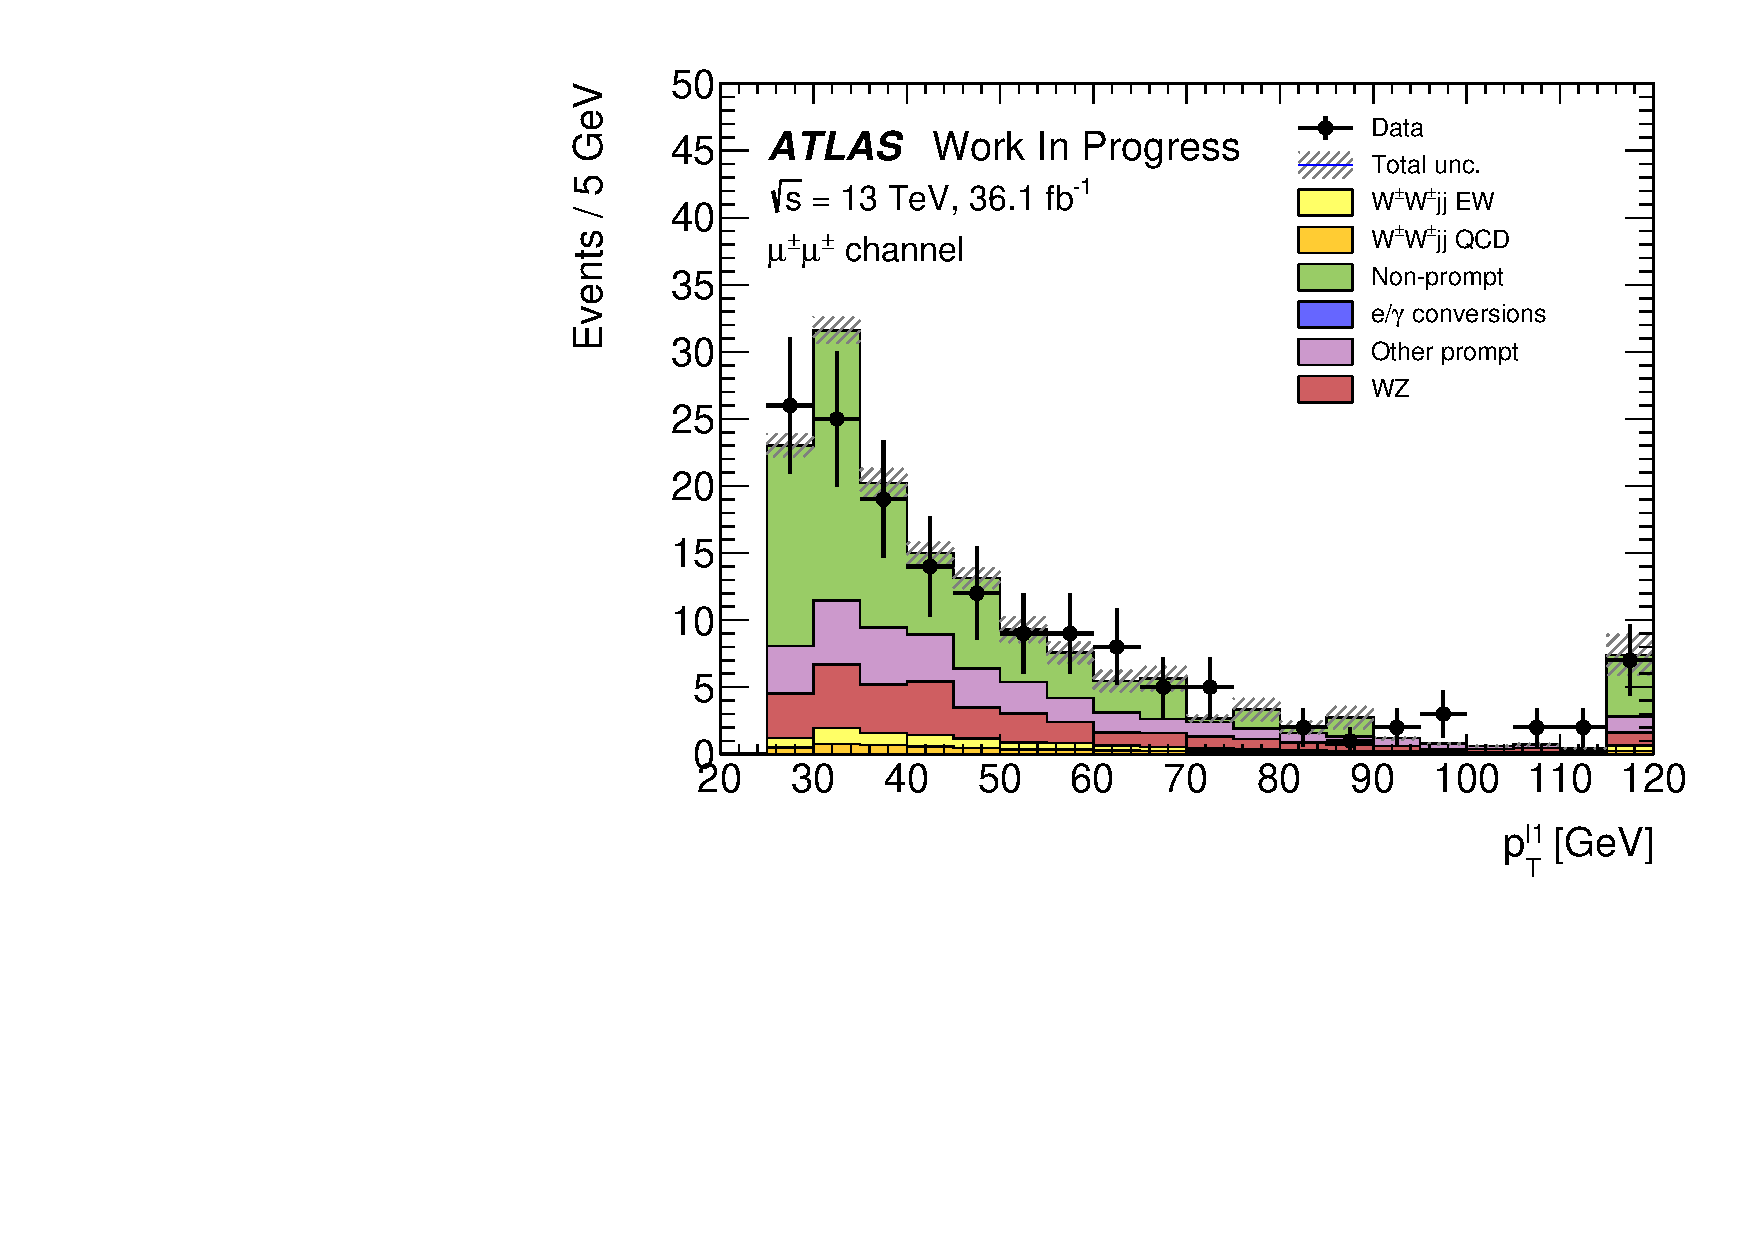
\includegraphics[width=.48\textwidth]{figs/ssww_13tev/backgrounds/ff/fakes_vr/mm-CutCRTopFakesSSZVeto-l1_pt-lin}
  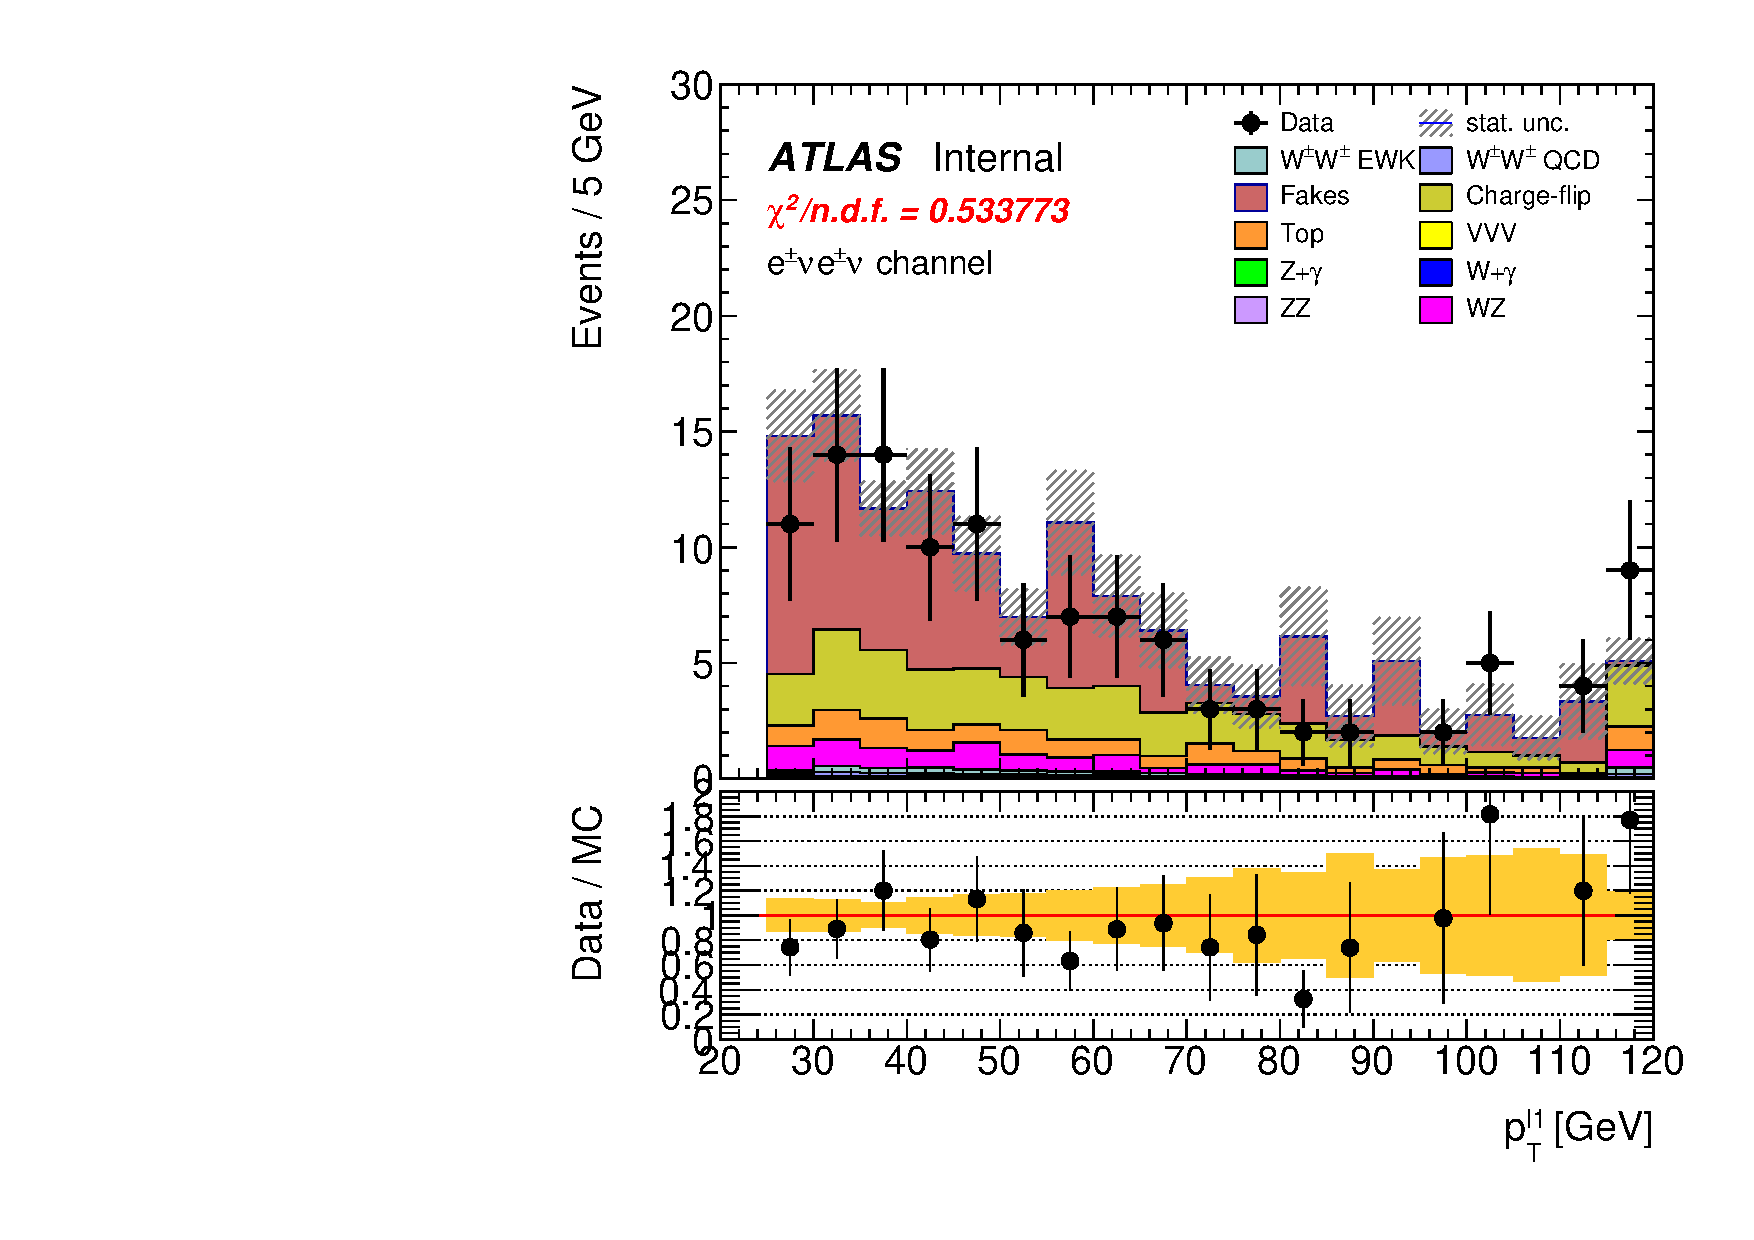
\includegraphics[width=.48\textwidth]{figs/ssww_13tev/backgrounds/ff/fakes_vr/ee-CutCRTopFakesSSZVeto-l1_pt-lin}\\
  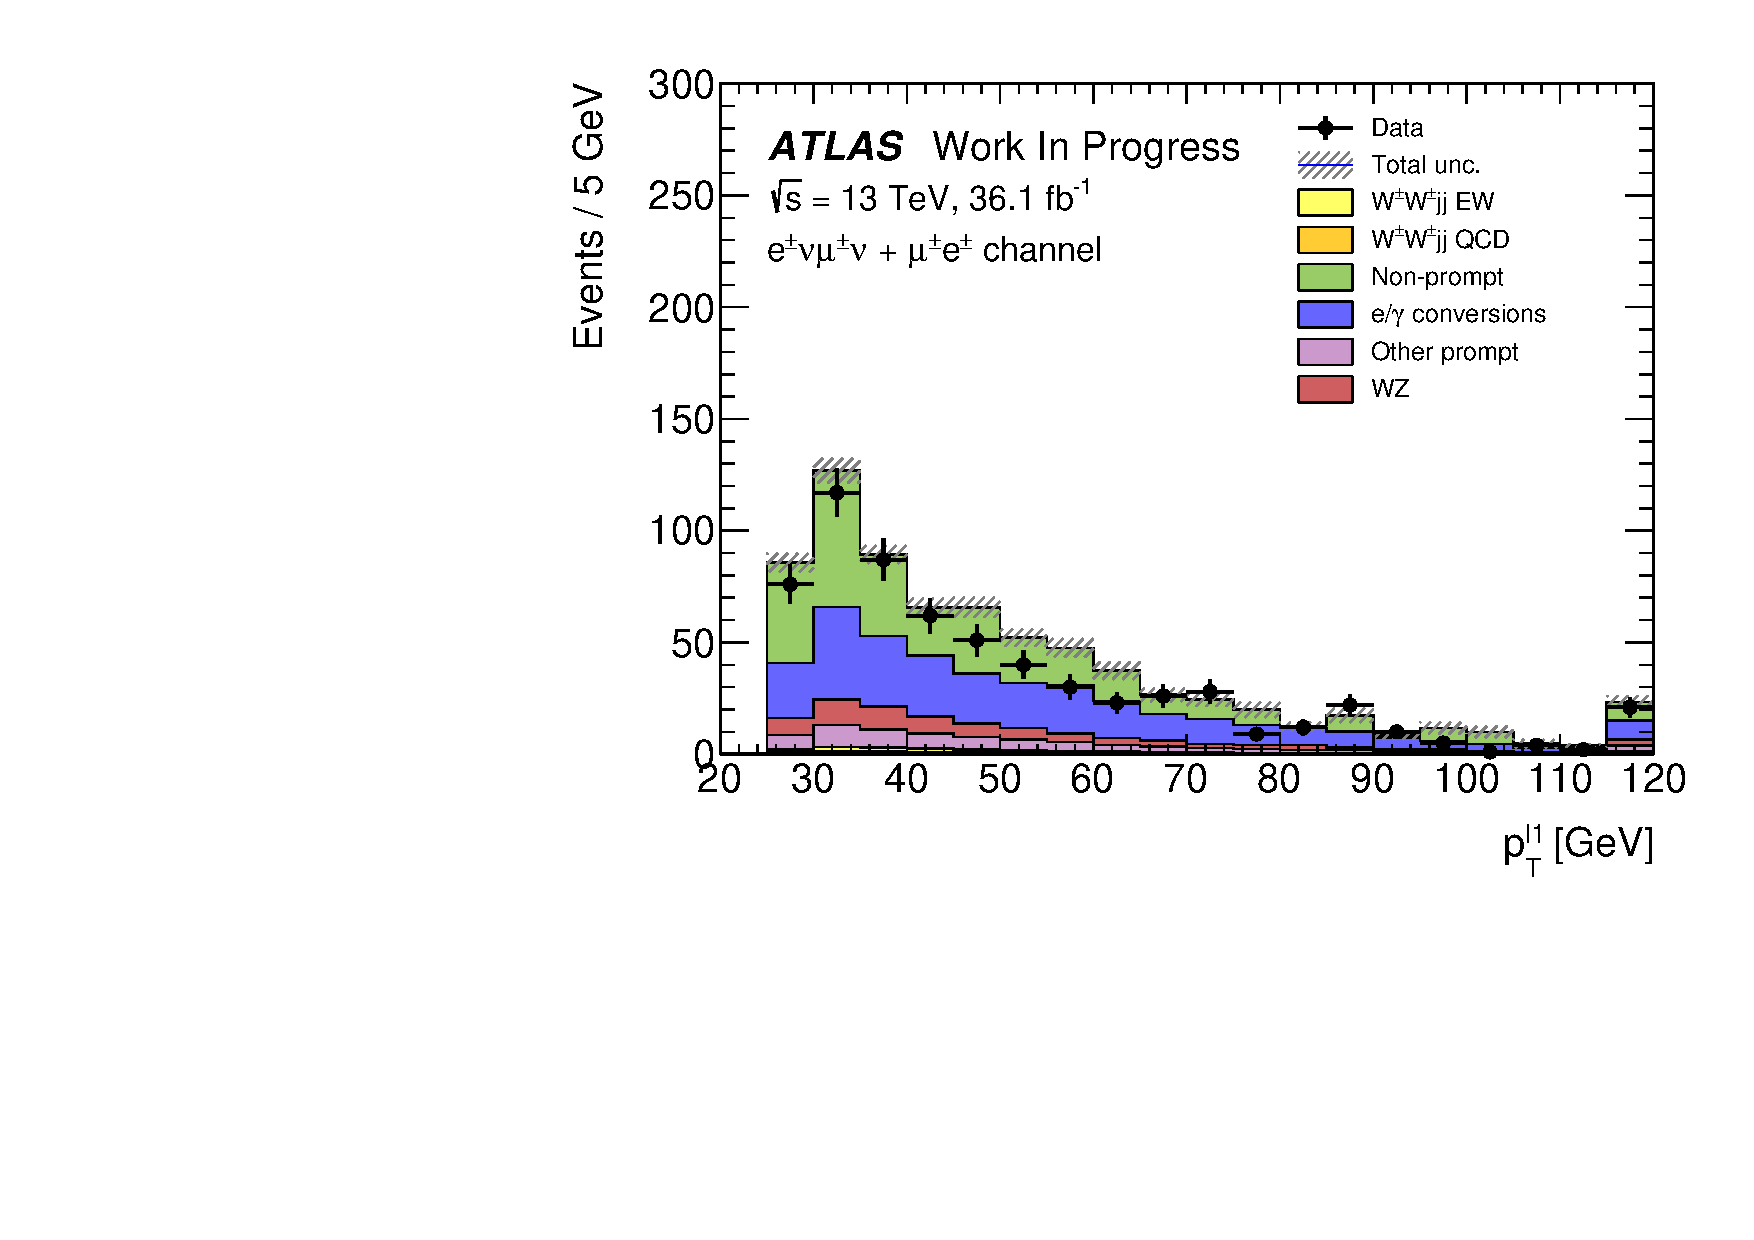
\includegraphics[width=.48\textwidth]{figs/ssww_13tev/backgrounds/ff/fakes_vr/emme-CutCRTopFakesSSZVeto-l1_pt-lin}
  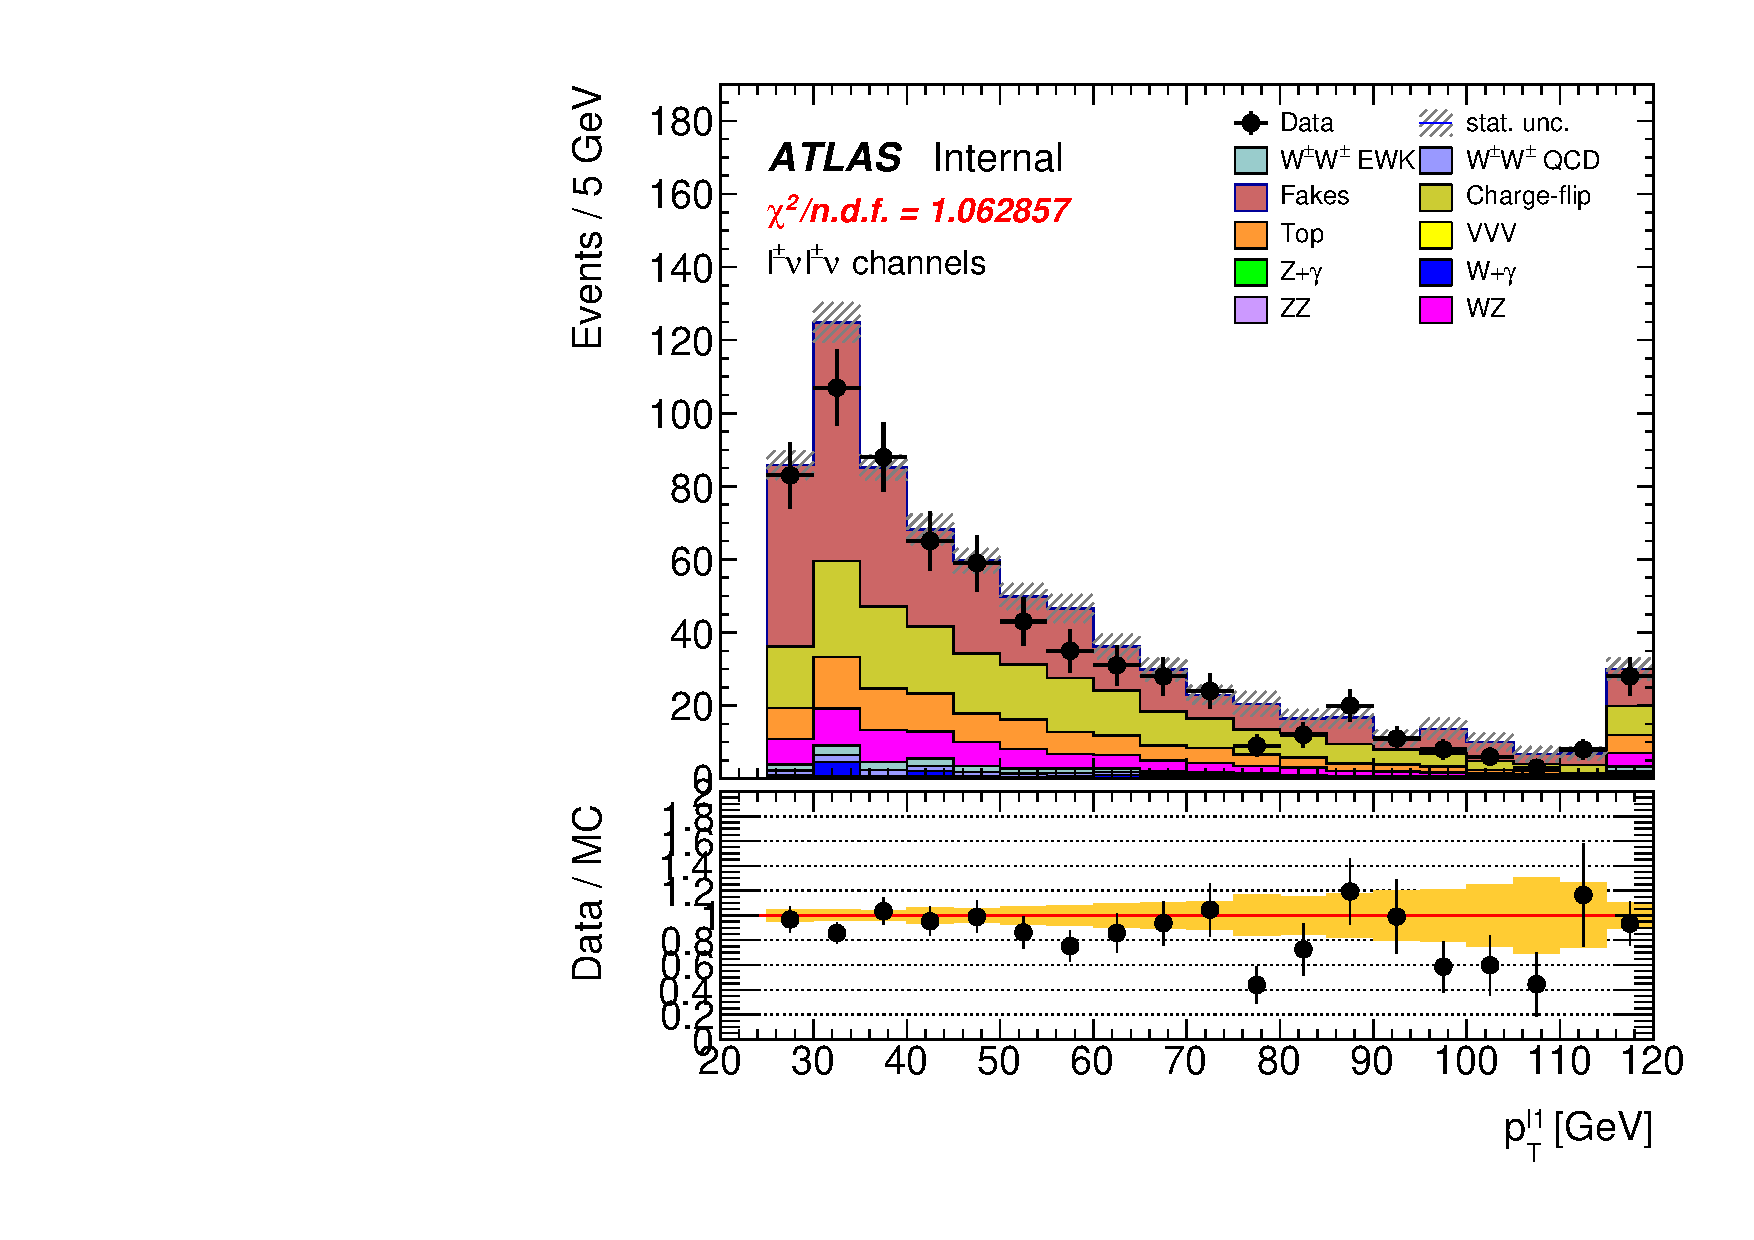
\includegraphics[width=.48\textwidth]{figs/ssww_13tev/backgrounds/ff/fakes_vr/ll-CutCRTopFakesSSZVeto-l1_pt-lin}
  \caption{Distributions of the subleading lepton $\pt$ in the same-sign top fakes VR for  $\mm$ events (top right), $\ee$ events (top left), $\me$ events (bottom left), and all events combined (bottom right).  All errors are statistical only.}
  \label{fig:ssww13tev_ff_fakes_vr}
\end{figure} 
